\documentclass[manuscript,screen,review]{acmart}

\AtBeginDocument{%
  \providecommand\BibTeX{{%
    Bib\TeX}}}

%% Rights management --- replace with values from your rights form
\setcopyright{acmlicensed}
\copyrightyear{2026}
\acmYear{2026}
\acmDOI{XXXXXXX.XXXXXXX}

%% Journal identifier --- REQUIRED for TALLIP
\acmJournal{TALLIP}

\begin{document}

\title[Gaokerena]{Gaokerena: A Small Persian Medical Language Model Family}

%% --- Authors and Affiliations ---

\author{Mehrdad Ghassabi}
\affiliation{%
  \institution{University of Isfahan}
  \city{Isfahan}
  \country{Iran}}

\author{Hamidreza Baradaran Kashani}
\affiliation{%
  \institution{University of Isfahan}
  \city{Isfahan}
  \country{Iran}}

\author{Pedram Rostami}
\affiliation{%
  \institution{University of Tehran}
  \city{Tehran}
  \country{Iran}}

\author{Sadra Hakim}
\affiliation{%
  \institution{University of Windsor}
  \city{Windsor}
  \state{ON}
  \country{Canada}}

\author{Zahra Kazemi}
\affiliation{%
  \institution{Alzahra University}
  \city{Tehran}
  \country{Iran}}

\author{Amirhossein Poursina}
\affiliation{%
  \institution{Isfahan University of Medical Sciences}
  \city{Isfahan}
  \country{Iran}}

\author{Milad Tavakoli}
\affiliation{%
  \institution{University of Isfahan}
  \city{Isfahan}
  \country{Iran}}

\author{Audrina Ebrahimi}
\affiliation{%
  \institution{University of Texas at Dallas}
  \city{Dallas}
  \state{TX}
  \country{USA}}
  \email{audrina.ebrahimi@utdallas.edu}
  \authornote{Corresponding author.}

\renewcommand{\shortauthors}{Ghassabi et al.}

%% --- Abstract ---

\begin{abstract}
Language resources for Persian medical natural language processing remain scarce, which limits the development of small medical language models for low-resource settings. We present Gaokerena, an open suite of Persian medical resources and two compact models built on them. The resources are: an 85.5-million-word corpus of 101,954 articles crawled from Persian medical magazines and health portals; MF3QA, a 24,000-pair patient--doctor question--answering dataset distilled from 186,029 raw forum pairs; a 2,967-question multiple-choice benchmark that brings together 1,878 items from the Iranian Basic Medical Science Entrance Exam (KOPP), 1,710 of them added in this article, and 1,089 translated MMLU medical items (FA\_MED\_MMLU); and an 18,000-question machine-translated MedMCQA training set filtered by two LLM referees. We characterise the corpus, MF3QA and the benchmarks in detail, including composition, orthography, redundancy, selection effects, privacy and sensitive content. Using these resources we train Gaokerena-V, by domain adaptation and instruction tuning, and Gaokerena-R, by preference-based reasoning distillation (RLAIF with DPO). On translated medical MMLU, Gaokerena-V reaches 49.31\% accuracy under direct prompting, against 46.65\% for its Aya-Expanse-8B backbone; this 2.66-point difference is not statistically significant ($p=0.21$). Gaokerena-R reaches 52.80\% with chain-of-thought prompting, five-sample self-consistency and a verifier tie-break, significantly above the directly prompted backbone ($p=0.004$) but at several times the inference cost. Under matched chain-of-thought self-consistency without the verifier, Gaokerena-R (48.7\%) is not significantly different from the backbone (46.9\%, $p=0.41$) but is clearly above Gaokerena-V (40.1\%). On the same questions in English the Aya-Expanse-8B backbone reaches 59.04\% (direct) and 63.18\% (CoT-SC), 12--16 points above its Persian accuracy; our resources and models narrow this gap but do not close it. These are single-run, unpaired comparisons, and we discuss their limits. Claim-level uncertainty heads for both models are summarised but reported elsewhere. All resources and models are openly released.
\end{abstract}

%% --- CCS Concepts ---
%% IDs below should be re-checked at https://dl.acm.org/ccs

\begin{CCSXML}
<ccs2012>
 <concept>
  <concept_id>10010147.10010178.10010179</concept_id>
  <concept_desc>Computing methodologies~Natural language processing</concept_desc>
  <concept_significance>500</concept_significance>
 </concept>
 <concept>
  <concept_id>10010147.10010257</concept_id>
  <concept_desc>Computing methodologies~Machine learning</concept_desc>
  <concept_significance>300</concept_significance>
 </concept>
 <concept>
  <concept_id>10010405.10010444.10010449</concept_id>
  <concept_desc>Applied computing~Health informatics</concept_desc>
  <concept_significance>300</concept_significance>
 </concept>
</ccs2012>
\end{CCSXML}

\ccsdesc[500]{Computing methodologies~Natural language processing}
\ccsdesc[300]{Computing methodologies~Machine learning}
\ccsdesc[300]{Applied computing~Health informatics}

\keywords{small medical language model, low-resource languages, Persian, reasoning language models, reinforcement learning with AI feedback}

\maketitle

%% ------------------------------------------------------------------
\section{Introduction}\label{sec1}

Language resources and models for Persian medical natural language processing (NLP) have only recently begun to emerge, with Gaokerena-V~\cite{b1}, Gaokerena-R~\cite{b2}, and claim-level uncertainty estimation for them~\cite{b3} among the first open efforts. The transformer architecture~\cite{b4} has driven rapid progress in NLP and the spread of large language models (LLMs) into high-stakes domains, including medicine, where they are used to support diagnosis, patient care and administrative workflows.

Modern language models range from a few billion parameters to architectures far larger. Large models offer broad knowledge and strong reasoning, but their computational requirements preclude deployment on consumer-grade local hardware. In clinical settings this creates privacy and data-security concerns, because sensitive patient information must often be sent to external servers. Small medical language models that can run locally on edge devices are therefore attractive.

English-centric small medical models exist, such as MedReason~\cite{b5}, but non-English languages are far less served. For Persian, to the best of our knowledge, the only existing medical language model at the beginning of this research was Sina-BERT~\cite{b6}, which is closed with respect to both weights and training data and is a non-generative encoder, which limits its use for conversational clinical tasks.

The scarcity of Persian medical data is, in part, a matter of under-use of existing digital assets. Persian medical forums (e.g., Drhast, Doctor-yab) and online medical magazines (e.g., Hidoctor, Niniban) host large repositories of expert-written content and authentic patient--doctor interactions. Annual high-stakes medical examinations are another untapped resource if they are extracted from legacy PDF formats. Translating established English medical datasets offers a further route to narrowing the gap.

This paper presents a suite of data resources and two open small language models for the Persian medical domain, \textbf{Gaokerena-V} and \textbf{Gaokerena-R}, the latter trained for step-by-step reasoning. We evaluate both on newly curated benchmarks and test the reported differences for statistical significance. All artefacts, including datasets, model weights and generated model responses, are available at \url{https://github.com/Mehrdadghassabi/Gaokerena-V} and \url{https://github.com/Mehrdadghassabi/Gaokerena-R}.

\paragraph{Relation to earlier publications.} This article extends our conference papers on Gaokerena-V~\cite{b1} and Gaokerena-R~\cite{b2}. Compared with them, it adds the characterisation of the medical corpus, MF3QA and the MCQ benchmarks (Sections~\ref{subsubsec:corpus_analysis}, \ref{subsubsec:mf3qa_analysis} and \ref{subsubsec:mcq_analysis}), 1,710 further KOPP questions (the conference papers used the September 2023 session only), which are released together with FA\_MED\_MMLU as one benchmark, a unified evaluation of both models with confidence intervals and significance tests, an English--Persian comparison (Section~\ref{subsec6.3}), and a summary of the uncertainty heads of~\cite{b3}. Some numbers differ from the conference versions, always by less than one percentage point, for two reasons. First, the pooled MMLU averages reported here are computed from question counts, whereas some averages in the conference papers did not exactly equal the pooled subject-level results (for example, 52.98\% in~\cite{b2} against 52.80\% here for Gaokerena-R with the verifier, and 46.28\% against 46.10\% for Gaokerena-R under straight prompting). Second, in the conference papers the chosen option was extracted from each model's raw response text by an automatic, AI-based step; for this article we manually rechecked these extractions and corrected some of them. The figures in this article supersede the earlier ones. The GPT-4o preference evaluation of free-form answers in~\cite{b1} is not repeated, because we subsequently found GPT-4o unreliable as a judge of Persian medical text. The matched chain-of-thought self-consistency results of~\cite{b2} are included in Section~\ref{subsec6.2} with significance tests.

The contributions are:

\begin{itemize}

    \item \textbf{A Persian medical corpus.} 101,954 articles (85.5 million words) crawled from Persian medical magazines and health portals, with an analysis of composition, orthography, redundancy, boilerplate and topical coverage.

    \item \textbf{The MF3QA dataset.} 24,000 patient--doctor question--answer pairs (23,799 originally Persian and 201 translated from K-QA), distilled from 186,029 raw forum pairs and split into 20,000 training, 2,000 development and 2,000 test pairs. We analyse split composition, selection effects, question--answer alignment, privacy exposure, sensitive content, duplication, topical coverage and overlap with the corpus.

    \item \textbf{An extended MCQ benchmark.} 2,967 questions: 1,878 from the Iranian Basic Medical Science Entrance Exam (KOPP), of which 168 (the September 2023 session) were used in our conference papers and 1,710 are added here, and 1,089 translated MMLU medical questions (FA\_MED\_MMLU, introduced in~\cite{b1}), released together, with an analysis of composition, answer-key balance, text quality, translation fidelity and duplication.

    \item \textbf{A translated MCQ training set.} About 18,000 Persian medical MCQs obtained by machine translation of MedMCQA and filtered by two LLM referees, intended for training only so that translation artefacts do not affect evaluation.

    \item \textbf{Two reasoning-distillation strategies} (Expert-Guided Synthesis and Iterative Self-Correction) used to train Gaokerena-R.

    \item \textbf{Two small Persian medical language models,} Gaokerena-V and Gaokerena-R, built on Aya-Expanse-8B. They are research artefacts and are not cleared for clinical use.

    \item \textbf{An English--Persian comparison.} The same questions and protocols applied to the backbone in English quantify the language gap and how much of it our resources and methods recover (Section~\ref{subsec6.3}).

\end{itemize}

%% ------------------------------------------------------------------
\section{Related Work}\label{sec2}

\subsection{English Small Medical Language Models}\label{subsec2.1}

Meerkat~\cite{b7} fine-tunes small models on medical Chain-of-Thought (CoT)~\cite{b8} reasoning paths extracted from medical textbooks together with complementary biomedical data, shifting the emphasis from factual recall to clinical decision-making processes.

MedS$^3$~\cite{b9} (referred to as MedSSS in earlier versions) pursues reasoning through search and process supervision. It applies Monte Carlo Tree Search over multiple-choice medical questions to generate step-by-step reasoning paths, yielding three synthetic datasets: a supervised fine-tuning set for the policy model, a preference set for reinforcement learning, and a soft-label set for a process reward model that guides generation by scoring intermediate steps.

MedMobile~\cite{b10} targets efficiency rather than reasoning. It fine-tunes Microsoft's Phi-3-mini~\cite{b11} on a blend of human-curated and synthetic medical data so that it can run on resource-constrained mobile devices without a persistent cloud connection.

\subsection{Persian Small Language Models}\label{subsec2.2}

Many multilingual models support Persian, but smaller variants often suffer from language mixing, grammatical errors and limited linguistic nuance, because Persian is a small fraction of their training data. Aya-Expanse~\cite{b12,b13} addresses this with a multilingual training recipe that relies partly on synthetic data from stronger models, giving it good Persian syntax and semantics; being general-purpose, it is weaker on specialised medical knowledge. PersianMind~\cite{b14} is an open bilingual Persian--English model built by extending the LLaMA-2~\cite{b15} tokenizer and continuing training. It is also general-purpose and has had no exposure to clinical corpora. Because Aya-Expanse was trained on a larger corpus and has better general knowledge, we chose it as the base for Gaokerena and focused on its medical deficiencies.

%% ------------------------------------------------------------------
\section{Data Collection}\label{sec3}

The Persian medical domain lacks both specialised small language models and research-grade datasets, so we assembled our own. The pipeline combines human and machine translation of foreign-language datasets, web scraping, and extraction of multiple-choice questions from PDF documents.

\subsection{Persian Medical Corpus}\label{subsec3.1}

Without domain-specific text, building Persian medical models is difficult. We compiled a corpus of 101,954 articles totalling 85.5 million words from Persian medical magazines and health portals.\footnote{\url{https://huggingface.co/datasets/gaokerena/medical_corpus}} Our earlier publication~\cite{b1} reported about 90M words for this corpus; the difference is due to the counting method. The earlier figure was the number of tokens returned by the Hazm word tokenizer on raw text, which includes punctuation marks as separate tokens, whereas the 85.5M figure counts only words after the normalisation and word-boundary rule described in Section~\ref{subsubsec:corpus_analysis}. Garc\'ia-Ferrero et al.~\cite{b16} compiled medical texts in four languages (English, French, Spanish and Italian); Table~\ref{corpus_comparison} compares sizes. The contribution of each source website is shown in Fig.~\ref{fig1}.

\begin{figure}[h]
\centering
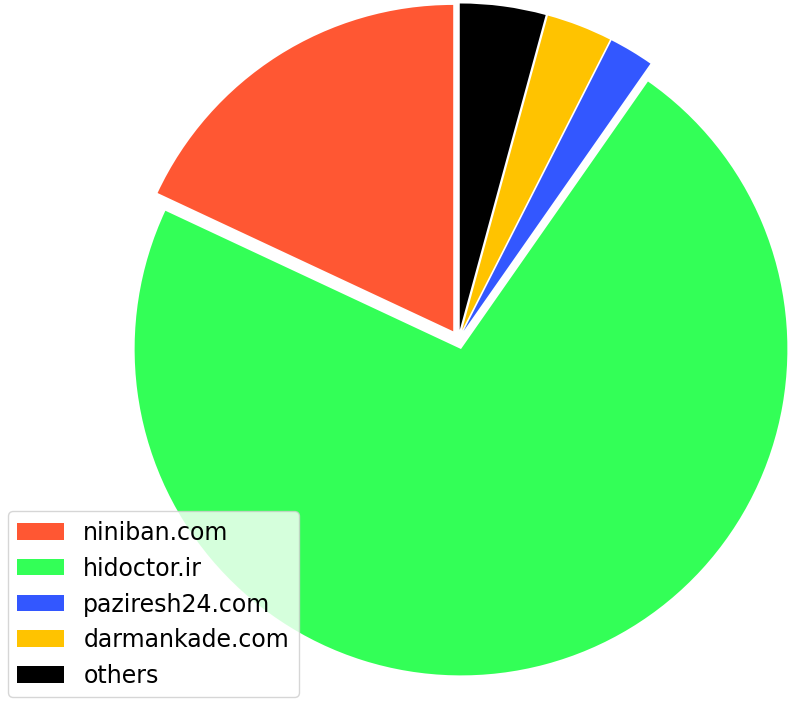
\includegraphics[width=0.5\textwidth]{fig1.png}
\caption{Medical corpus sources}\label{fig1}
\Description{Bar chart showing the distribution of articles across 11 Persian medical websites, with hidoctor.ir dominating at 72.3 percent.}
\end{figure}

\begin{table}[h]
\caption{Comparison of our corpus with corpora collected by Garc\'ia-Ferrero et al. (token counts as reported by them; our corpus is measured in words, so the comparison is only indicative).}\label{corpus_comparison}
\begin{tabular}{@{}lcl@{}}
\toprule
Language & Size & Collected by \\
\midrule
English & 1.1B & Garc\'ia-Ferrero et al. \\
Spanish & 950M & Garc\'ia-Ferrero et al. \\
French  & 675M & Garc\'ia-Ferrero et al. \\
Italian & 143M & Garc\'ia-Ferrero et al. \\
Persian & 85.5M & This work \\
\bottomrule
\end{tabular}
\end{table}

\subsubsection{Corpus Characteristics}\label{subsubsec:corpus_analysis}

We analysed composition, orthographic quality, redundancy, boilerplate content and topical coverage. Word counts are computed on text normalised for Persian/Arabic character variants, digits and punctuation, with the zero-width non-joiner (ZWNJ) treated as a word boundary.

\textbf{Composition.} The corpus has 101,954 articles from 11 websites, 85.5M words and 417M characters. The median article has 620 words (5th--95th percentile: 128--2,198). As Table~\ref{tab:corpus_sources} and Fig.~\ref{fig10} show, a few sources dominate: hidoctor.ir supplies 72.3\% of articles and 62.0\% of words, and the two largest sources together supply 80.7\% of words. Articles from most smaller sources are longer (median 1,013--2,246 words, against 527 for hidoctor.ir; niniban.com at 737 and salammag.com at 882 are the exceptions). Very short articles are rare (502 articles, 0.5\%, have fewer than 50 words), as are very long ones (four exceed 10,000 words).

\begin{table}[h]
\caption{Composition of the Persian medical corpus by source. Dup.\ is the share of articles flagged as exact or near duplicates; Boiler.\ is the mean share of an article's characters made up of sentences that recur in at least 20 articles.}\label{tab:corpus_sources}
\begin{tabular}{@{}lrrrrr@{}}
\toprule
Source & Articles & Words (M) & Median words & Dup.\ (\%) & Boiler.\ (\%) \\
\midrule
hidoctor.ir & 73,668 & 52.98 & 527 & 1.3 & 0.8 \\
niniban.com & 18,389 & 16.04 & 737 & 13.5 & 4.6 \\
darmankade.com & 3,316 & 5.90 & 1,731 & 13.1 & 2.9 \\
paziresh24.com & 2,259 & 3.43 & 1,307 & 0.0 & 9.2 \\
doctoreto.com & 2,071 & 4.38 & 2,246 & 0.2 & 1.4 \\
salammag.com & 787 & 0.77 & 882 & 0.0 & 4.3 \\
seebmagazine.com & 452 & 0.59 & 1,332 & 1.8 & 0.1 \\
majalepezeshki.ir & 322 & 0.41 & 1,183 & 0.0 & 0.0 \\
hamrah-teb.com & 312 & 0.45 & 1,506 & 0.0 & 0.4 \\
nabz.site & 270 & 0.42 & 1,555 & 0.0 & 0.0 \\
extern.ir & 108 & 0.13 & 1,013 & 0.9 & 0.0 \\
\midrule
Total & 101,954 & 85.50 & 620 & 3.8 & 1.8 \\
\bottomrule
\end{tabular}
\end{table}

\begin{figure}[h]
\centering
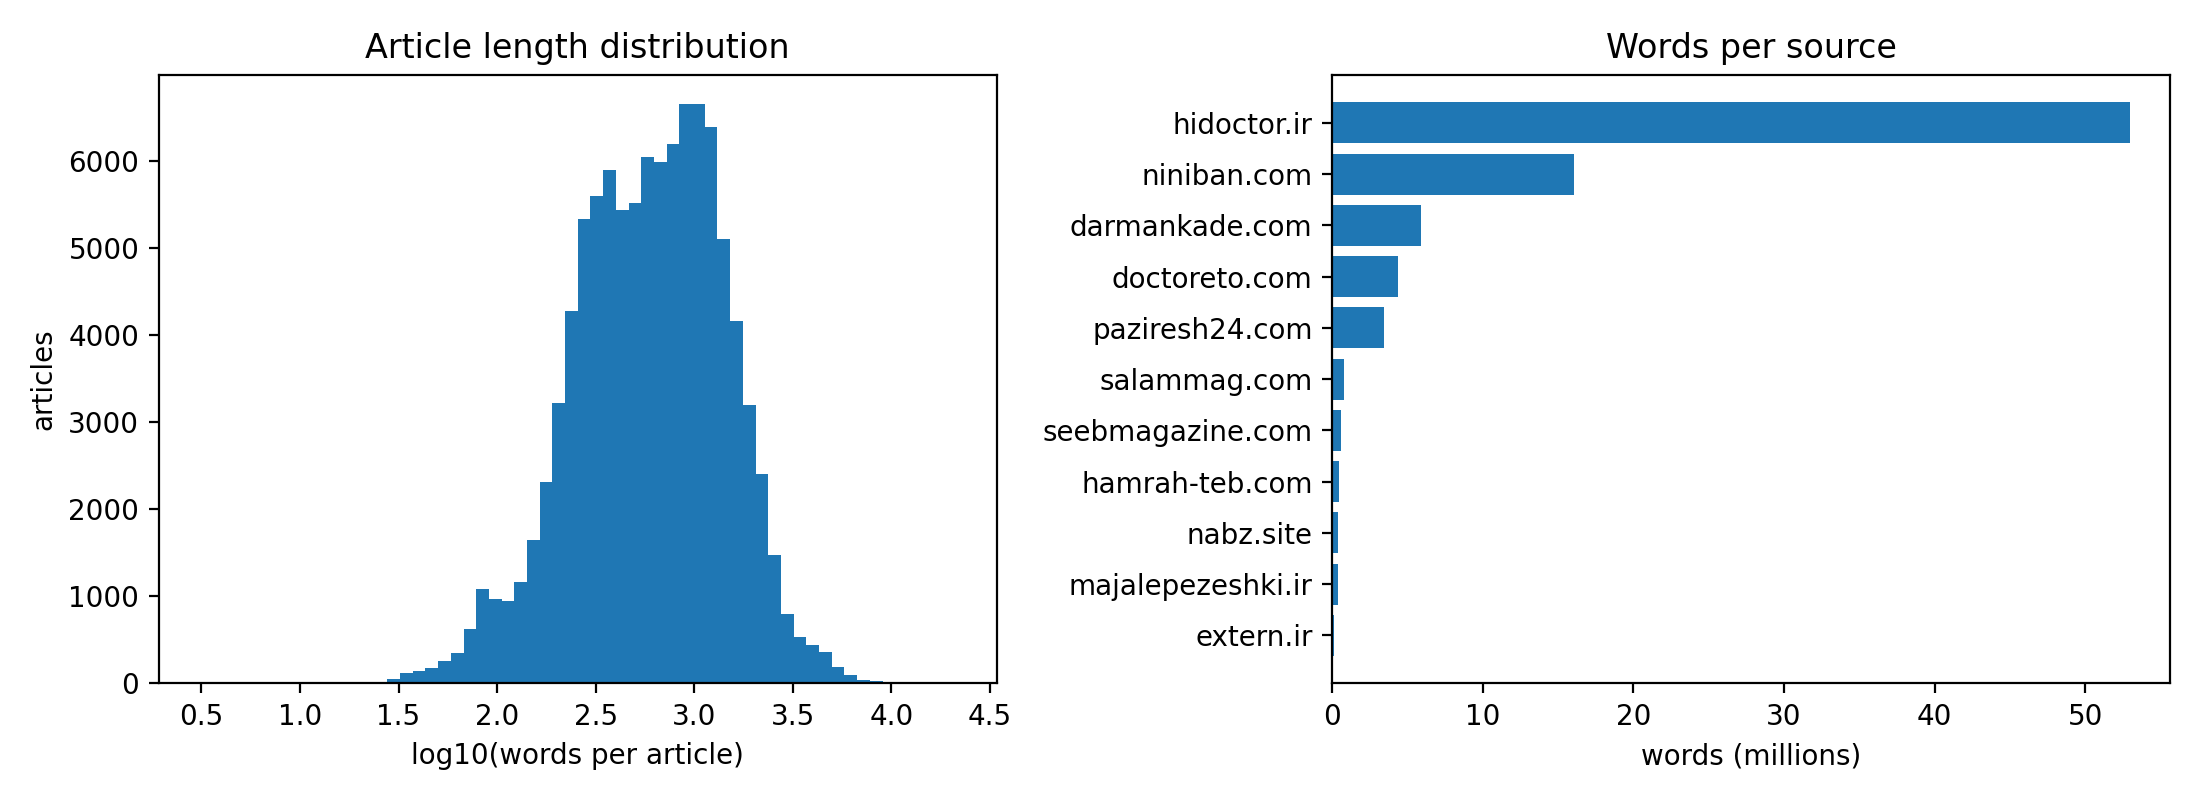
\includegraphics[width=\textwidth]{fig10.png}
\caption{Article length distribution (left) and words per source (right) in the Persian medical corpus}\label{fig10}
\Description{Two-panel figure showing the distribution of article lengths and the total word count per source in the Persian medical corpus.}
\end{figure}

\textbf{Script and orthography.} Persian/Arabic-script letters make up 96.6\% of non-whitespace characters and Latin letters 0.6\%; only 36 articles (0.04\%) are more than 20\% Latin. Orthography is nevertheless not uniform. Arabic Yeh or Kaf (instead of the Persian forms) appears in 7.0\% of articles, 88\% of which come from hidoctor.ir; 14.0\% of articles mix Persian and ASCII digits; and ZWNJ frequency ranges from 19 per 1,000 words (extern.ir) to 96 (nabz.site), reflecting different editorial conventions. This fragments the surface forms a tokenizer sees, so we recommend character normalisation before training.

\textbf{Redundancy.} After normalisation, 2,257 articles (2.2\%) are exact duplicates of an earlier article and 3,903 (3.8\%, including the exact duplicates) are exact or near duplicates, detected by MinHash LSH on 5-word shingles of the first 500 words with a Jaccard threshold of 0.8. Redundancy is concentrated in niniban.com (13.5\%) and darmankade.com (13.1\%), against 1.3\% for hidoctor.ir. Exact duplication across sources is negligible (13 articles), but 423 articles have a near-duplicate in a different source, consistent with syndicated or lightly rewritten content. Removing all flagged articles leaves 98,051 articles and 80.7M words (a 5.6\% reduction in words).

\textbf{Boilerplate and provenance.} A total of 2,193 distinct sentences occur in at least 20 articles. On average they make up 1.8\% of an article's characters, and 4,542 articles (4.5\%) exceed 10\%, with the highest mean shares in paziresh24.com (9.2\%), niniban.com (4.6\%) and salammag.com (4.3\%). The most frequent sentences are reuse and attribution footers, promotional calls to action (e.g., booking or online consultation prompts) and standard drug-leaflet warnings. They also show that parts of the corpus are not original professional authorship: a magazine's translation-team credit appears in 1,521 articles, a ``translated and rewritten by'' credit in 618, and a news-agency credit in 977 (counts are per sentence and may overlap).

\textbf{Topical coverage.} We fitted a 15-component TF-IDF/NMF topic model on a random sample of 20,000 articles and assigned each article to its dominant topic (Table~\ref{tab:corpus_topics}; labels were assigned manually from the top terms). Coverage is broad across clinical areas, with general symptoms and conditions, cardiovascular disease and diabetes, and sleep and mental health the largest groups. A non-trivial part is only loosely medical: cooking recipes (5.4\%) and directory listings of laboratories and clinics (2.7\%) together make up about 8\% of the sample, alongside cosmetics (6.5\%) and general lifestyle content. Topic mixes differ by source; niniban.com, for example, is dominated by pregnancy, childcare and sexual-health topics.

\begin{table}[h]
\caption{Dominant topics in a 20,000-article sample of the corpus (NMF, 15 components)}\label{tab:corpus_topics}
\begin{tabular}{@{}lr@{}}
\toprule
Topic & Articles (\%) \\
\midrule
Symptoms, infections and surgery & 14.9 \\
Cardiovascular disease, diabetes and research news & 12.3 \\
Sleep, mental health and lifestyle & 12.0 \\
Diet and nutrition & 8.0 \\
Infant and child care, breastfeeding & 6.8 \\
Skin, hair and cosmetics & 6.5 \\
Medications & 5.9 \\
Sexual health and infertility & 5.9 \\
Pregnancy and fetal development & 5.7 \\
Cooking recipes & 5.4 \\
Cancer & 4.2 \\
Vitamins, minerals and supplements & 3.9 \\
Childbirth and delivery & 3.2 \\
Directory listings (labs, clinics, addresses) & 2.7 \\
Dental and oral health & 2.6 \\
\bottomrule
\end{tabular}
\end{table}

%% ------------------------------------------------------------------
\subsection{MF3QA}\label{subsec3.2}

Real doctor--patient question--answer data helps language models learn medical terminology, patient concerns and the structure and tone of professional replies. Despite reputable Persian forums such as Drhast, no comprehensive Persian dataset of this kind existed at the start of this work, so we introduce what we believe is the first Medical Free-Form Farsi Question Answering dataset (MF3QA).\footnote{\url{https://huggingface.co/datasets/gaokerena/MF3QA}. The raw crawl before cleaning is at \url{https://huggingface.co/datasets/gaokerena/MF3QA_uncleaned}.} The survey of Liu et al.~\cite{b17} lists several real doctor--patient QA datasets; Table~\ref{mf3qa_comparison} compares them with MF3QA.

\begin{table}[h]
\caption{Comparison of our dataset with existing medical QA datasets}\label{mf3qa_comparison}
\begin{tabular}{@{}llc@{}}
\toprule
Dataset name & Language & No. records \\
\midrule
ChatDoctor~\cite{b18} & English & 100K \\
CMtMedQA~\cite{b19} & Chinese & 68K \\
DISC-Med-SFT~\cite{b20} & Chinese & 465K \\
HuatuoGPT-sft-data-v1~\cite{b21} & Chinese & 226K \\
Huatuo-26M~\cite{b22} & Chinese & 26M \\
MedDialog~\cite{b23} & Chinese \& English & 3.66M \\
Medical-Meadow~\cite{b24} & English & 160K \\
MF3QA (this work) & Persian & 24K \\
\bottomrule
\end{tabular}
\end{table}

We crawled 186,029 raw question--answer (QA) pairs from prominent Persian medical forums (Fig.~\ref{fig2}) and cleaned them with a hybrid pipeline of automated filtering and manual verification. The approach follows ChatDoctor~\cite{b18}, in which roughly half of the scraped English pairs were discarded by answer length because truncated answers can limit a model's ability to generate full explanations. Persian practitioners online answer much more briefly than their English-speaking counterparts, so the filtering is much more aggressive here: about 87\% of raw records were removed (186,029 reduced to 24,000).

The pipeline has several stages. To shift the token-count distribution towards longer, more informative answers, before the filtering began we randomly dropped a portion of the short answers (fewer than 50 tokens) from the training and development pools. The filtering steps below were applied after this step, and the combined effect behaves as a length floor (see Section~\ref{subsubsec:mf3qa_analysis}). The random omission was not applied to the test split. Instead, every QA pair in the test set was reviewed for factual accuracy and clinical validity. For the test split we also used data from the Doctor-yab and Isovisit platforms and added a translation of the K-QA dataset~\cite{b25} to increase diversity. Training and development records were additionally screened for spam and low-quality entries. We also removed any personal data to ensure compliance with privacy standards. The result is 20,000 training, 2,000 development and 2,000 test pairs. Section~\ref{subsubsec:mf3qa_analysis} quantifies the consequences of this selection.

Drhast exposes only its 2,000 most recent dynamic records, and each record links to about 100 related entries. We modelled the site as a graph and ran repeated Breadth-First Search (BFS) traversals, using newly posted records as fresh roots in later runs and skipping records already visited. This extracted 120,000 records out of an estimated 200,000 in two weeks.

\begin{figure}[h]
\centering
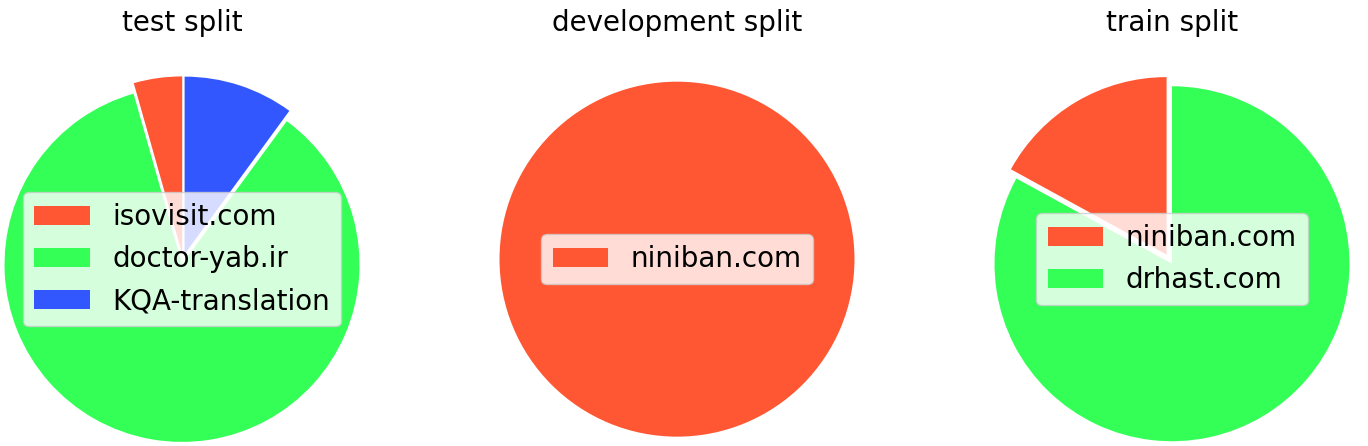
\includegraphics[width=\textwidth]{fig2.png}
\caption{MF3QA sources}\label{fig2}
\Description{Pie chart showing the proportion of question-answer pairs collected from each Persian medical forum.}
\end{figure}

\subsubsection{MF3QA Characteristics}\label{subsubsec:mf3qa_analysis}

We analysed the cleaned dataset (24,000 pairs) against its raw crawl (186,029 pairs) along these dimensions: split composition, selection effects of cleaning, token counts, question--answer alignment, answer style, privacy exposure, sensitive content, duplication and leakage, topical coverage, and overlap with the corpus of Section~\ref{subsec3.1}. Lengths are in words on text normalised as for the corpus. Several screens (style, personal data, sensitive content, topics) are keyword- or regular-expression-based heuristics that flag items for review; their counts are approximate, and we did not manually validate their precision. Privacy and sensitive-content percentages are computed over questions unless stated otherwise.

\textbf{Split composition.} The splits come from different sources (Table~\ref{tab:mf3qa_splits}). Training combines Drhast (83.0\%) and Niniban (17.0\%); development is entirely Niniban; test is Doctor-yab (85.6\%), Isovisit (4.4\%) and the 201 translated K-QA items (10.1\%). Source is therefore fully confounded with split, and the development split is not drawn from the test distribution. The distributions also differ in length (Fig.~\ref{fig11}): the median test question has 11 words against 51 in training and 45 in development, and two-sample Kolmogorov--Smirnov tests between training and test give $D=0.55$ for question length and $D=0.33$ for answer length ($p<10^{-170}$ for both). The test split therefore measures out-of-distribution generalisation relative to training, and results on it should be reported per source.

\begin{table}[h]
\caption{MF3QA composition by split and source. Lengths are in words; ``Raw'' is the uncleaned crawl before filtering.}\label{tab:mf3qa_splits}
\begin{tabular}{@{}llrrrr@{}}
\toprule
Split & Source & Rows & Q median & A median & A mean \\
\midrule
Train & drhast.com & 16,596 & 53 & 57 & 70.7 \\
Train & niniban.com & 3,404 & 46 & 76 & 97.5 \\
Dev & niniban.com & 2,000 & 45 & 77 & 97.8 \\
Test & doctor-yab.ir & 1,711 & 11 & 48 & 58.3 \\
Test & isovisit.com & 88 & 38 & 37 & 43.7 \\
Test & K-QA (translated) & 201 & 9 & 100 & 103.3 \\
\midrule
Raw & all four sources & 186,029 & 43 & 17 & 25.9 \\
\bottomrule
\end{tabular}
\end{table}

\begin{figure}[h]
\centering
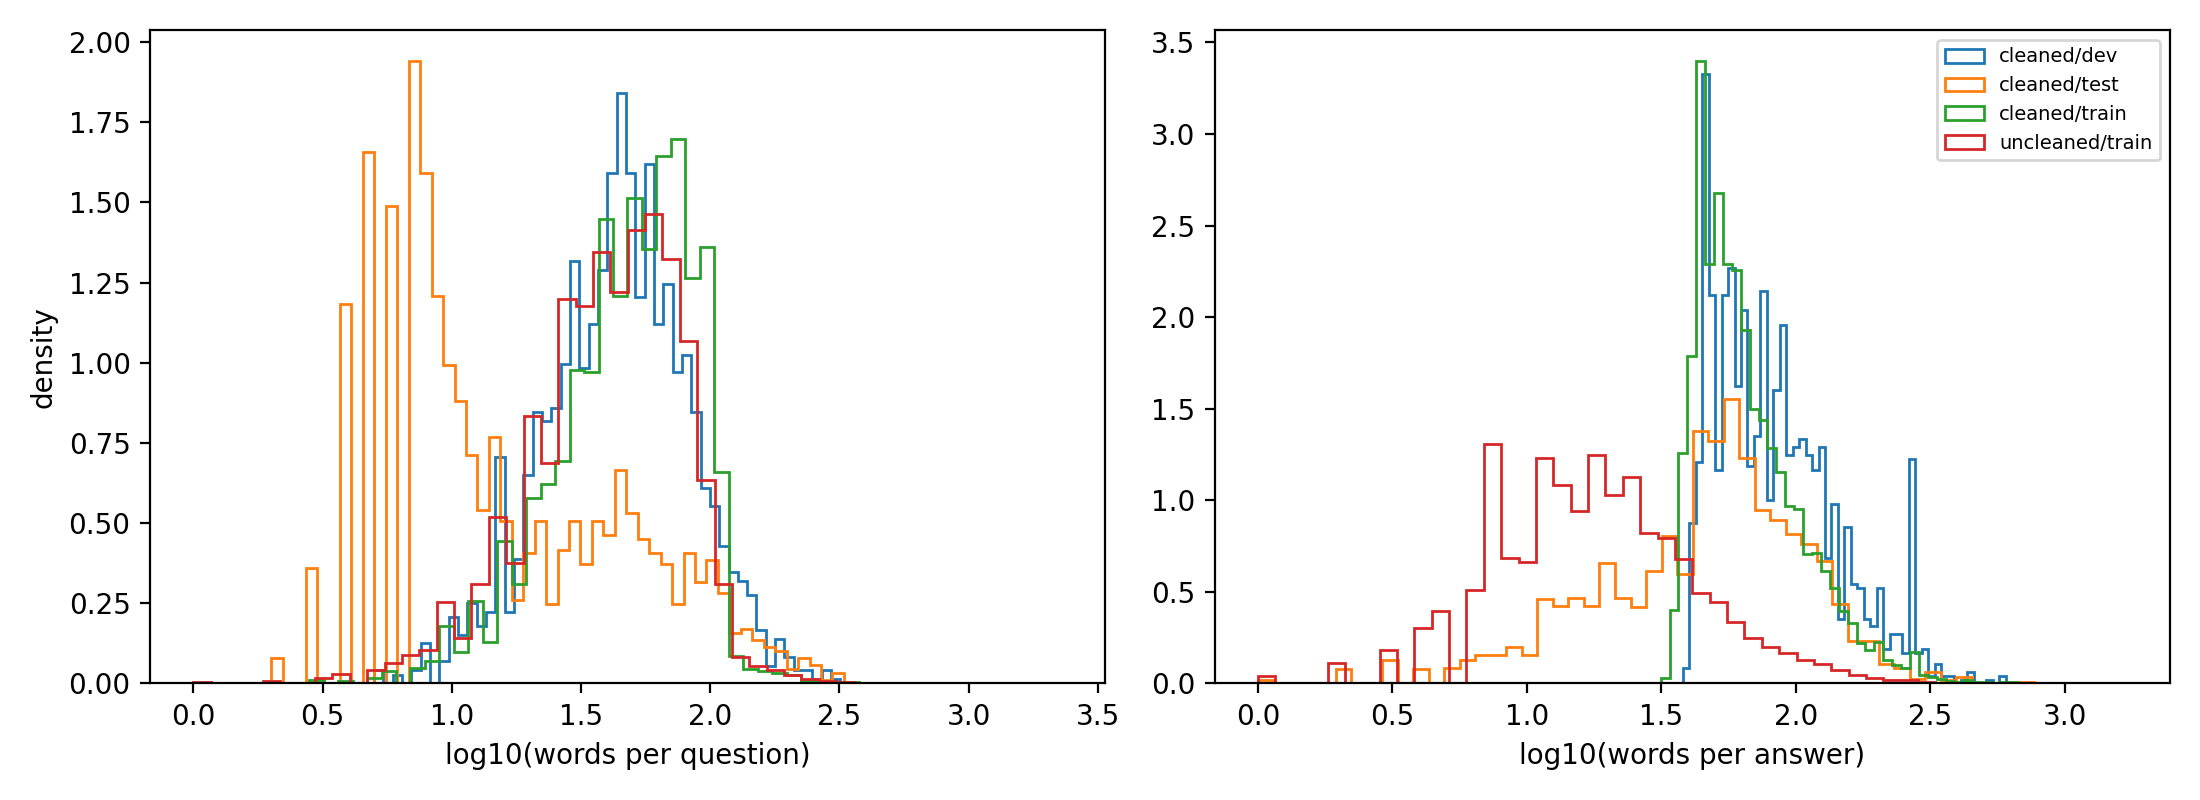
\includegraphics[width=\textwidth]{fig11.png}
\caption{Distribution of question length (left) and answer length (right), in words on a log scale, for the MF3QA splits and the uncleaned crawl}\label{fig11}
\Description{Two-panel violin or box plots showing the distribution of question and answer lengths across MF3QA splits and the raw crawl.}
\end{figure}

\textbf{Selection effects of cleaning.} Cleaning retained 24,000 of 186,029 raw pairs, and its effect is dominated by answer length (Table~\ref{tab:mf3qa_funnel}). The median raw answer has 17 words, 74.3\% of raw answers are shorter than 30 words, and 13.2\% are short (at most 15 words) referral-only replies that tell the patient to see a physician. Of the raw pairs with answers of at most 25 words (127,454, or 68.5\% of the crawl), 0.4\% were retained, against 80.6\% of those with more than 50 words; question length has only a weak relationship with retention (9.5--20.2\% across length bins). Retention also differs sharply by source (Drhast 13.6\%, Doctor-yab 3.1\%, Niniban 58.9\%), and Doctor-yab contributes only to the test split. As a result, training and development answers are almost never short (0.015\% and 0.0\% under 30 words, and none under 50 tokens), whereas 27.9\% of test answers have fewer than 30 words because the random omission was not applied there; in practice the random omission followed by filtering behaves as a near-deterministic length floor in training and development. Models fine-tuned on MF3QA are consequently exposed to longer and more elaborate replies than are typical of the forums from which it was drawn, and test-set outputs should not be compared with training-style answer lengths without accounting for this. The raw crawl also contains scraping artefacts (83 pairs with an empty question or answer, repeated browser-error and media-player strings, and recurring clinic advertisements), which the length filter removes. All 23,799 originally Persian pairs were matched to a raw record by normalised question text; the 201 translated K-QA items are absent from the crawl by construction. The per-source kept counts in Table~\ref{tab:mf3qa_funnel} total 23,799 Persian pairs, or 24,000 with the 201 translated K-QA items, and equal the per-source split sizes in Table~\ref{tab:mf3qa_splits} (for example, 1,711 Doctor-yab test pairs).

\begin{table}[h]
\caption{Survival of raw MF3QA records through cleaning, by source and by answer length (matched on normalised question text). The 201 translated K-QA items are not in the crawl and are added to the by-source kept total.}\label{tab:mf3qa_funnel}
\begin{tabular}{@{}lrrr@{}}
\toprule
 & Raw & Kept & Kept (\%) \\
\midrule
\multicolumn{4}{@{}l}{\emph{By source}} \\
drhast.com & 122,233 & 16,596 & 13.57 \\
doctor-yab.ir & 54,539 & 1,711 & 3.13 \\
niniban.com & 9,172 & 5,404 & 58.88 \\
isovisit.com & 88 & 88 & 100.0 \\
K-QA (translated) & --- & 201 & --- \\
\midrule
Total kept & & 24,000 & \\
\midrule
\multicolumn{4}{@{}l}{\emph{By answer length (words)}} \\
$\leq$10 & 50,504 & 146 & 0.3 \\
11--25 & 76,950 & 359 & 0.5 \\
26--50 & 38,783 & 7,173 & 18.5 \\
51--100 & 14,585 & 11,561 & 79.3 \\
101--200 & 4,386 & 3,645 & 83.1 \\
$>$200 & 821 & 738 & 89.9 \\
\bottomrule
\end{tabular}
\end{table}

\textbf{Token counts.} Token counts depend strongly on the tokenizer. With the Qwen2.5 tokenizer the training split contains 7.28M tokens (3.18M in questions and 4.10M in answers; 2.72 tokens per answer word), the development split 0.82M and the test split 0.51M. Median answer length is 163, 204 and 135 tokens for training, development and test, and 14.95\% of test answers (but no training or development answers) are shorter than 50 tokens. Counts under other tokenizers, including the Aya-Expanse tokenizer used for training, will differ.

\textbf{Question--answer alignment.} To check for mismatched pairs, we scored each pair by the cosine similarity of multilingual sentence embeddings (paraphrase-multilingual-MiniLM-L12-v2, texts truncated to 600 characters) and compared it with the similarity of randomly re-paired questions and answers (Fig.~\ref{fig12}). True pairs are clearly more similar than random pairs (mean 0.53 against 0.24), but the distributions overlap. Using the median of the random-pair distribution as a conservative threshold, 938 pairs (3.9\%) are flagged as likely mismatches (training 3.9\%, development 2.9\%, test 4.6\%); by source the rate is 2.5\% for Niniban, 4.2\% for Drhast, 4.6\% for Doctor-yab, 3.0\% for K-QA and 8.0\% for Isovisit (88 pairs). A looser criterion, similarity below the 95th percentile of random pairs, flags 36.2\% of pairs (41.3\% for Doctor-yab); this is expected because its questions are very short and doctors' replies are often generic, and it should not be read as an error rate. Because the embedding model is general-purpose, flagged pairs are candidates for manual inspection, not confirmed errors.

\begin{figure}[h]
\centering
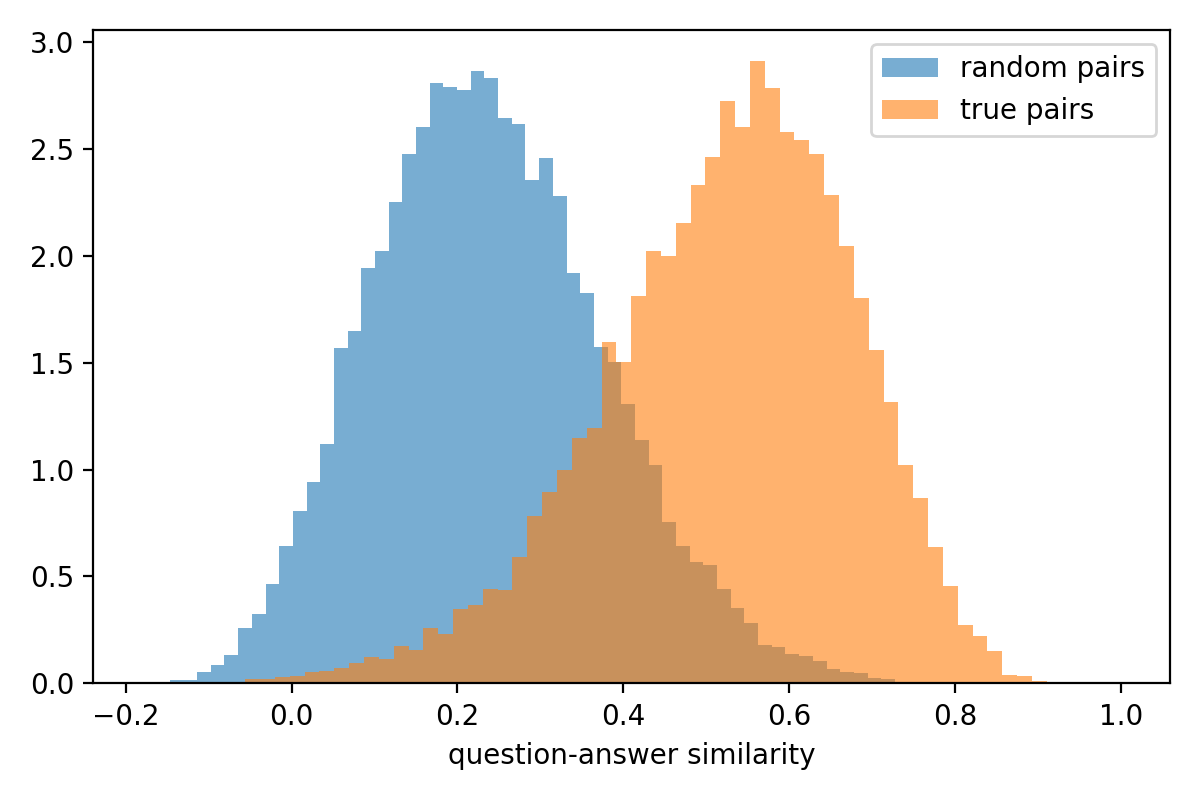
\includegraphics[width=0.7\textwidth]{fig12.png}
\caption{Question--answer similarity for true pairs and for randomly shuffled pairs in MF3QA}\label{fig12}
\Description{Histogram showing the cosine similarity distribution for true question-answer pairs versus randomly shuffled pairs.}
\end{figure}

\textbf{Style and provenance.} We used lexical proxies for answer style: stock formal phrases typical of generated text, colloquial verb forms, greetings and ZWNJ density. A combined ``LLM-like'' flag (a stock phrase, or a ZWNJ-rich formal register with no colloquial forms in answers of at least 60 words) fires on 10.3\% of pairs, stock phrases alone on 7.9\% and colloquial forms on 15.3\%. Flag rates are highest for the translated K-QA items (40.3\%, with 27.9\% stock phrases and no colloquial forms), consistent with translated text, and are 9.0\% for Drhast, 12.4\% for Niniban, 15.4\% for Doctor-yab and 1.1\% for Isovisit. Register differs systematically by source: Niniban answers are formal (0.3\% contain colloquial forms and none starts with a greeting), whereas Drhast answers are colloquial (20.2\%) and mostly open with a greeting (69.0\%). Within the training split the flag rate varies between 5.3\% and 13.7\% across position deciles with no monotonic trend. Formal phrases such as ``it is recommended'' are also common in human medical writing, so we do not read these rates as evidence of machine generation; they show that the register of the supervision signal depends on the source.

\textbf{Duplication and leakage.} The cleaning pipeline did not include a deduplication step, so we measured the duplication that remains in the released data. Exact duplication is rare: 17 training questions (0.09\%), one development question and none in the test split repeat an earlier question in the same split, and 11 training and one development pairs repeat an earlier question--answer pair in full. Three development questions also occur in training (two with identical answers), and no test question occurs in either of the other splits. With MinHash LSH on 3-word shingles of questions of at least five words (Jaccard threshold 0.8) we find about 77 near-duplicate question pairs inside training, one inside development, one inside test, and 10 development questions with a near-duplicate in training; no test question has a near-duplicate in training. The nearest training question to a test question has a median TF-IDF cosine similarity of 0.16 (95th percentile 0.34), and one test question (0.05\%) reaches 0.8, against 16 development questions (0.8\%). Train--test leakage through near-duplicate questions is therefore negligible, and train--development leakage is small. Answers are more repetitive than questions: 3.7\% of cleaned pairs share their answer with at least four other pairs. The most frequent answer occurs 118 times and is a canned reply on fetal sex selection; the most repeated answers are dominated by pregnancy and emergency-contraception replies. Some recommend home procedures for which we know of no supporting evidence, which shows that a physician-authored source does not guarantee that every answer is clinically sound, and that a model trained on MF3QA will reproduce frequently repeated content most strongly.

\textbf{Personal data.} Apart from the personal-data removal applied during cleaning (Section~\ref{subsec3.2}), the text is distributed as it appeared on public pages, so we screened for residual direct contact details with regular expressions (URLs, e-mail addresses, mobile and landline numbers, social-media handles). Cleaning removed most of them: among raw answers, 1.08\% contain a mobile number, 0.58\% a landline number, 0.41\% a URL and 0.08\% a social handle (largely clinic advertisements), whereas the cleaned dataset has at most 18 of 24,000 pairs with any of these (12 through the question: 11 in training and one e-mail address in development; 6 through the answer: four in training and two in test). Named physicians are a separate category: a regex for a name following ``Dr.'' fires on 12.8\%, 9.2\% and 5.7\% of training, development and test questions, and on 2.8\%, 10.5\% and 0.4\% of answers respectively. This detector is approximate and over-counts (for example, forms of address), but answers do contain physician signature lines and questions may name treating physicians. We applied no further anonymisation, and users who need a stricter release should filter or mask these items; the screening script exports row identifiers rather than the matched values.

\textbf{Sensitive content.} Patient questions cover intimate and high-risk topics (Table~\ref{tab:mf3qa_sensitive}). Keyword screens flag a self-harm term in 0.6\% of training questions (119) and 0.7\% of test questions (14), a first-person age below 18 in 0.8\% of training and 1.3\% of test questions, a child together with a dosing term in 5.6\% of training questions (1,111), and sexual-health terms in 4.2\%. Rates in the raw crawl are of the same order, so cleaning did not remove this content. The development split is a special case: 55.9\% of its questions mention pregnancy, against 17.0\% in training and 2.8\% in test, a consequence of its coming only from Niniban. Pediatric dosing is a particular hazard for generated advice because errors can cause direct harm, and a model fine-tuned on this data has had no safety-specific filtering of such cases. We therefore advise against using MF3QA-trained models for dosing advice and recommend manual review of flagged questions, with a content note for users, before any broader release.

\begin{table}[h]
\caption{Keyword-screen flags on MF3QA questions (\% of questions; counts in parentheses). Screens are heuristic and over- and under-count.}\label{tab:mf3qa_sensitive}
\small
\begin{tabular}{@{}lrrrr@{}}
\toprule
Flag & Train & Dev & Test & Raw crawl \\
\midrule
Rows & 20,000 & 2,000 & 2,000 & 186,029 \\
Self-harm term & 0.6 (119) & 0.0 (0) & 0.7 (14) & 0.5 (868) \\
First-person age $<$18 & 0.8 (154) & 0.5 (10) & 1.3 (25) & 1.1 (2,117) \\
Child + dosing term & 5.6 (1,111) & 7.9 (158) & 1.1 (22) & 3.9 (7,320) \\
Sexual-health term & 4.2 (840) & 6.7 (133) & 3.1 (62) & 6.9 (12,758) \\
Pregnancy term & 17.0 (3,405) & 55.9 (1,118) & 2.8 (56) & 15.7 (29,117) \\
\bottomrule
\end{tabular}
\end{table}

\textbf{Topical coverage.} A 12-component TF-IDF/NMF model fitted on a random sample of 20,000 of the 24,000 pairs (questions and answers concatenated; labels assigned manually from top terms) shows that the splits cover different content (Table~\ref{tab:mf3qa_topics}). The first topic is better described as an informal, first-person register (relationships, sexual concerns, general complaints) than as a medical subject. Reproductive-health topics (conception, contraception and menstruation, pregnancy, childbirth, pregnancy tests, infertility) account for 22.6\% of the training sample, 69.8\% of the development sample and 11.0\% of the test sample, whereas general diagnosis, treatment and surgery accounts for 40.0\% of the test sample but only 12.3\% of training and 1.9\% of development. The topic gap between development and test, like the gap in length, is a reason not to use the development split as a proxy for test performance.

\begin{table}[h]
\caption{Dominant topics in a 20,000-pair sample of MF3QA (NMF, 12 components): share of the sample overall and within each split (\%).}\label{tab:mf3qa_topics}
\small
\begin{tabular}{@{}lrrrr@{}}
\toprule
Topic & All & Train & Dev & Test \\
\midrule
Informal first-person narratives (relationships, general) & 23.5 & 26.1 & 5.1 & 14.9 \\
General diagnosis, treatment and surgery & 13.7 & 12.3 & 1.9 & 40.0 \\
Pain and physical complaints (dental, chest, back) & 13.2 & 14.1 & 3.3 & 14.8 \\
Medication use & 11.7 & 12.7 & 4.4 & 8.7 \\
Infertility and pregnancy planning & 7.5 & 6.5 & 22.2 & 2.4 \\
Weight, diet and growth & 6.7 & 6.6 & 4.6 & 9.7 \\
Pregnancy monitoring and miscarriage & 5.7 & 5.1 & 14.8 & 2.4 \\
Infant feeding and newborn care & 5.6 & 5.5 & 10.9 & 1.0 \\
Menstrual delay and pregnancy tests & 5.6 & 5.3 & 10.2 & 3.5 \\
Childbirth and caesarean & 3.0 & 2.6 & 8.7 & 1.8 \\
Ovulation and conception & 2.2 & 1.8 & 7.6 & 0.3 \\
Emergency contraception and menstrual disturbance & 1.7 & 1.3 & 6.4 & 0.6 \\
\bottomrule
\end{tabular}
\end{table}

\textbf{Overlap with the medical corpus.} Gaokerena-V is trained on both the corpus and MF3QA, so we measured how much MF3QA text also occurs in the corpus, using 8-gram overlap on normalised question--answer text against all 101,954 articles (an upper bound on what the model saw, since only 60\% of the corpus was used for domain adaptation). Some overlap is expected from shared boilerplate, so we report two thresholds. At least one shared 8-gram occurs in 14.6\% of training, 41.0\% of development and 18.5\% of test pairs; for 2.2\%, 11.7\% and 2.1\% of pairs respectively, more than half of the pair's 8-grams also occur in the corpus, a stronger indication of copied or syndicated content. The elevated development figures coincide with the development split's coming entirely from Niniban, which is also a corpus source (Table~\ref{tab:corpus_sources}); we did not verify the origin of individual matches. The main results of this paper use the MCQ benchmarks of Section~\ref{subsec3.3} and are not affected, but a free-form evaluation on the MF3QA development split after domain adaptation would not be independent of the training data, and about 2\% of test pairs (roughly 40) should be excluded or reported separately in such an evaluation.

\textbf{Implications for use.} MF3QA is best used as an instruction-tuning resource whose training distribution (longer, selected answers from Drhast and Niniban) differs deliberately from its test distribution (shorter questions, mostly Doctor-yab, plus translated items). We recommend reporting test results per source, treating the development split as source-specific, filtering or masking the flagged personal-data and near-duplicate rows, reviewing flagged sensitive and mismatched pairs before deployment-oriented use, and bearing in mind that frequently repeated answers are over-represented in the training signal.

%% ------------------------------------------------------------------
\subsection{Persian Medical Multiple Choice Question Dataset}\label{subsec3.3}

Multiple-choice question (MCQ) datasets complement free-form QA. Some training recipes, such as that of MedS$^3$~\cite{b9}, require MCQ data for instruction tuning, and MCQ accuracy offers an objective, quantifiable measure of a model's diagnostic and pharmacological knowledge, although it is only a partial proxy for clinical competence.

We curated two evaluation sets. First, we extracted 1,878 questions from the Iranian Basic Medical Science Entrance Exams (2021--2024) and converted them from PDF to a structured format (KOPP).\footnote{\url{https://huggingface.co/datasets/gaokerena/KOPP}} The September 2023 session (168 questions) was already used in our conference papers~\cite{b1,b2}; the other 1,710 questions are added in this article. Second, we manually translated the medical portion of the Massive Multitask Language Understanding (MMLU) dataset~\cite{b26}, 1,089 questions, to allow comparison with global benchmarks (FA\_MED\_MMLU),\footnote{\url{https://huggingface.co/datasets/gaokerena/FA_MED_MMLU}} which was introduced in~\cite{b1}.

Training data tolerates minor semantic variation better than evaluation data, so for training we used a scalable machine-translation pipeline. No comprehensive Persian medical MCQ dataset existed at the time, so we used DeepSeek-V3~\cite{b27} to translate a portion of MedMCQA~\cite{b28} from English to Persian.\footnote{\url{https://github.com/Mehrdadghassabi/Gaokerena-R/tree/main/dataset/medmcqa_translation_filterd}} Questions were sampled randomly from MedMCQA to cover disciplines such as physiology, pharmacology, pathology and clinical practice. For quality control, two independent LLM referees, Grok-3-mini~\cite{b29} and GPT-4.1-mini~\cite{b30}, scored each translated question and its options for semantic accuracy, fluency and preservation of medical terminology. A translation was accepted only if both referees gave a perfect score of five out of five, which yielded about 18,000 Persian MCQs. These scores are LLM judgements and were not validated against human annotators.

\subsubsection{MCQ Benchmark Characteristics}\label{subsubsec:mcq_analysis}

We analysed the released versions of KOPP and FA\_MED\_MMLU for size and composition, subject coverage, answer-key and format properties, text quality, translation fidelity and duplication. The text-quality and answer-length screens are regular-expression heuristics whose counts are approximate; we did not manually validate their precision.

\textbf{Size and composition.} The released KOPP contains 1,878 four-option questions, split into \texttt{sept23} (168 items, the September 2023 session) and \texttt{other\_years} (1,710 items). FA\_MED\_MMLU contains 1,089 items in six subject splits whose sizes (Table~\ref{tab:mcq_composition}) equal those of the English MMLU test sets for the same subjects, so the translation covers the complete test partition of each subject. Together the two benchmarks contain 2,967 questions. All items are single-answer with exactly four options, so chance is 25\%.

\begin{table}[h]
\caption{Composition of the MCQ benchmarks.}\label{tab:mcq_composition}
\begin{tabular}{@{}llrr@{}}
\toprule
Benchmark & Split / subject & Items & Share (\%) \\
\midrule
KOPP & sept23 & 168 & 8.9 \\
KOPP & other\_years & 1,710 & 91.1 \\
KOPP & all & 1,878 & 100.0 \\
\midrule
FA\_MED\_MMLU & anatomy & 135 & 12.4 \\
FA\_MED\_MMLU & clinical knowledge & 265 & 24.3 \\
FA\_MED\_MMLU & college biology & 144 & 13.2 \\
FA\_MED\_MMLU & college medicine & 173 & 15.9 \\
FA\_MED\_MMLU & medical genetics & 100 & 9.2 \\
FA\_MED\_MMLU & professional medicine & 272 & 25.0 \\
FA\_MED\_MMLU & all & 1,089 & 100.0 \\
\bottomrule
\end{tabular}
\end{table}

\textbf{Subject coverage.} The \texttt{sept23} split spans 9 subjects: anatomy (32.1\%, 54 items), physiology (21.4\%), biochemistry and principles of health services (11.9\% each), bacteriology (9.5\%), parasitology (6.0\%), virology and mycology (3.0\% each) and entomology (1.2\%, 2 items), so several subjects are too small to report separately. The remaining sessions cover 17 subjects after merging spelling variants, led by anatomy (27.0\%), physiology (17.9\%), bacteriology (10.8\%) and biochemistry (9.9\%), and including immunology, pathology, genetics, clinical psychology, epidemiology and medical physics, which do not occur in \texttt{sept23}. In FA\_MED\_MMLU, professional medicine and clinical knowledge together make up 49.3\% of items (537 of 1,089), so any pooled statistic is dominated by these two subjects and per-subject reporting is more informative.

\textbf{Answer key and format.} The correct option is in position 1/2/3/4 for 32.1/26.8/16.1/25.0\% of KOPP \texttt{sept23} items, 27.3/24.6/25.0/23.2\% of \texttt{other\_years} items and 21.6/23.3/22.8/32.3\% of FA\_MED\_MMLU items. The departure from a uniform key is significant for \texttt{sept23} (chi-square $p=0.029$; option 3 is correct for only 16.1\%) and strongly so for FA\_MED\_MMLU ($p=5.7\times10^{-7}$; option 4 is correct for 32.3\%), but not for \texttt{other\_years} ($p=0.12$). A constant-position guess therefore reaches 32.1\%, 27.3\% and 32.3\% respectively, above the nominal 25\% chance level; we did not check whether the FA\_MED\_MMLU skew is inherited from the English source. Option length gives no cue: the unique longest option is correct for 23.2\%, 20.8\% and 25.3\% of items (ties excluded). KOPP stems have a median of 13 words and options of 2 words, against 17 and 4 in FA\_MED\_MMLU. The two releases use different schemas (an integer answer index in KOPP, a string label in FA\_MED\_MMLU), which we recommend harmonising in a future version.

\textbf{Text quality.} KOPP was extracted from PDF exam booklets, and a manual read of the first page of the dataset viewer for \texttt{sept23} shows artefacts typical of automatic extraction of right-to-left text with embedded Latin and numerals: (i) numerals reordered or truncated, so that quantitative items are not answerable as written (an arterial blood-gas item gives pH ``64.7'' and $\mathrm{P_{CO_2}}$ ``.7'', and an ECG item gives a mean QRS axis ``31-'' and a voltage sum ``.41''); (ii) a stem replaced by a copy of an option from the preceding item; (iii) stray text appended to a stem; (iv) unbalanced parentheses; (v) missing whitespace at Persian--Latin boundaries; and (vi) mixed Arabic and Persian forms of Yeh and Kaf, the same variation reported for the corpus in Section~\ref{subsubsec:corpus_analysis}. These were found by inspection and are not an estimate of prevalence. Over all 1,878 KOPP items, heuristic screens flag 4 items (0.2\%) with reordered or truncated numerals, 2 (0.1\%) whose stem equals an option of the same or the preceding item, 13 (0.7\%) with duplicate options, 5 (0.3\%) with unbalanced parentheses in the stem (option-level truncations are not covered), 124 (6.6\%) with no whitespace at a Persian--Latin boundary, and 605 (32.2\%) with Arabic Yeh or Kaf; the last rate is 62.5\% in \texttt{sept23} against 29.2\% in the other sessions, so orthography differs by exam session. Latin letters occur in the stem of 20.4\% of items. Subject labels are affected too: the 17 distinct KOPP subjects appear under 24 strings because of Arabic/Persian letter variants and invisible directional control characters inherited from the PDFs. In FA\_MED\_MMLU the same screens flag 0.4\% (numerals), 0.2\% (duplicate options), 1.6\% (script boundary) and 0.7\% (Arabic Yeh or Kaf) of items, in line with its being translated rather than extracted text. The screens detect only specific patterns, so we recommend reviewing the exported flagged items before the benchmark is used for fine-grained comparison.

\textbf{Translation fidelity.} FA\_MED\_MMLU inherits the properties of its English source. Translated items show the usual artefacts: anatomical and clinical terms are sometimes left in Latin script (e.g., \emph{levator veli palatini}), transliterated, or translated inconsistently across options of one item, and some ambiguities of the English wording are not preserved in Persian. We did not perform a back-translation or second-annotator audit; we recommend a stratified audit across the six subjects reporting the rate of items whose key changes meaning under translation. Annotation errors present in the English MMLU medical subsets are carried over, and the key of a translated item should not be assumed to be more reliable than the original.

\textbf{Duplication.} Matching on normalised stems alone, 95 distinct stems occur more than once among the 2,967 items, and 199 stem pairs have a character $n$-gram TF--IDF cosine of at least 0.8, of which 6 pairs are between KOPP and FA\_MED\_MMLU. Because only stems are compared, short generic stems can match despite different options, so these counts are upper bounds on true duplicates; the flagged identifiers are exported for review.

\textbf{Implications for use.} KOPP is a small, session-structured benchmark whose \texttt{sept23} split has only 168 items, and FA\_MED\_MMLU is a complete translated test partition dominated by two subjects. We recommend reporting results per subject and per session, and excluding or repairing the flagged items (or reporting with and without them).

%% ------------------------------------------------------------------
\section{Gaokerena Models}\label{sec4}

Both models are built on Aya-Expanse-8B~\cite{b12,b13}. Gaokerena-V~\cite{b1} is obtained by domain adaptation on a subset of our corpus followed by instruction tuning on MF3QA. Gaokerena-R~\cite{b2} is post-trained on MCQs to distil medical reasoning from a larger teacher model.

\subsection{Gaokerena-V}\label{subsec4.1}

We adapt the 8B Aya-Expanse checkpoint in two LoRA~\cite{b31} stages (hyperparameters in Table~\ref{ft_it_training_details}), training on about 54 million new words in total (the conference version~\cite{b1} reported 57 million tokens, counted with the earlier tokenizer-based method explained in Section~\ref{subsec3.1}). In the domain-adaptation stage we continue pre-training on 60\% of the medical corpus (roughly 51M of its 85.5M words) to expose the model to Persian medical terminology; LoRA keeps the update lightweight and limits forgetting (loss in Fig.~\ref{fig3}). In the instruction-tuning stage we use the full MF3QA training split to refine conversational and QA behaviour, with a lower LoRA rank and alpha and a higher dropout rate to limit overfitting (loss in Fig.~\ref{fig4}). As Section~\ref{subsubsec:mf3qa_analysis} shows, this split is source-selected and length-filtered, and at most about 2\% of its pairs overlap heavily with the domain-adaptation corpus.

\begin{table}[h]
\caption{Gaokerena-V training hyperparameters}\label{ft_it_training_details}
\begin{tabular}{@{}lcc@{}}
\toprule
 & Domain adaptation & Instruction tuning \\
\midrule
Training data & medical\_corpus & MF3QA \\
Number of epochs & 1 & 1 \\
Batch size & 2 & 2 \\
Gradient accumulation steps & 16 & 16 \\
Optimizer & AdamW & AdamW \\
Learning rate & 5E-4 & 5E-4 \\
Maximum gradient norm & 0.3 & 0.3 \\
Warmup ratio & 0.03 & 0.03 \\
Weight decay rate & 0.1 & 0.5 \\
Maximum context length & 1024 & 1024 \\
Padding strategy & left-side padding & left-side padding \\
LoRA rank & 8 & 2 \\
LoRA alpha & 16 & 2 \\
LoRA dropout rate & 0.05 & 0.4 \\
Target modules & all linear layers & all linear layers \\
\bottomrule
\end{tabular}
\end{table}

\begin{figure}[h]
\centering
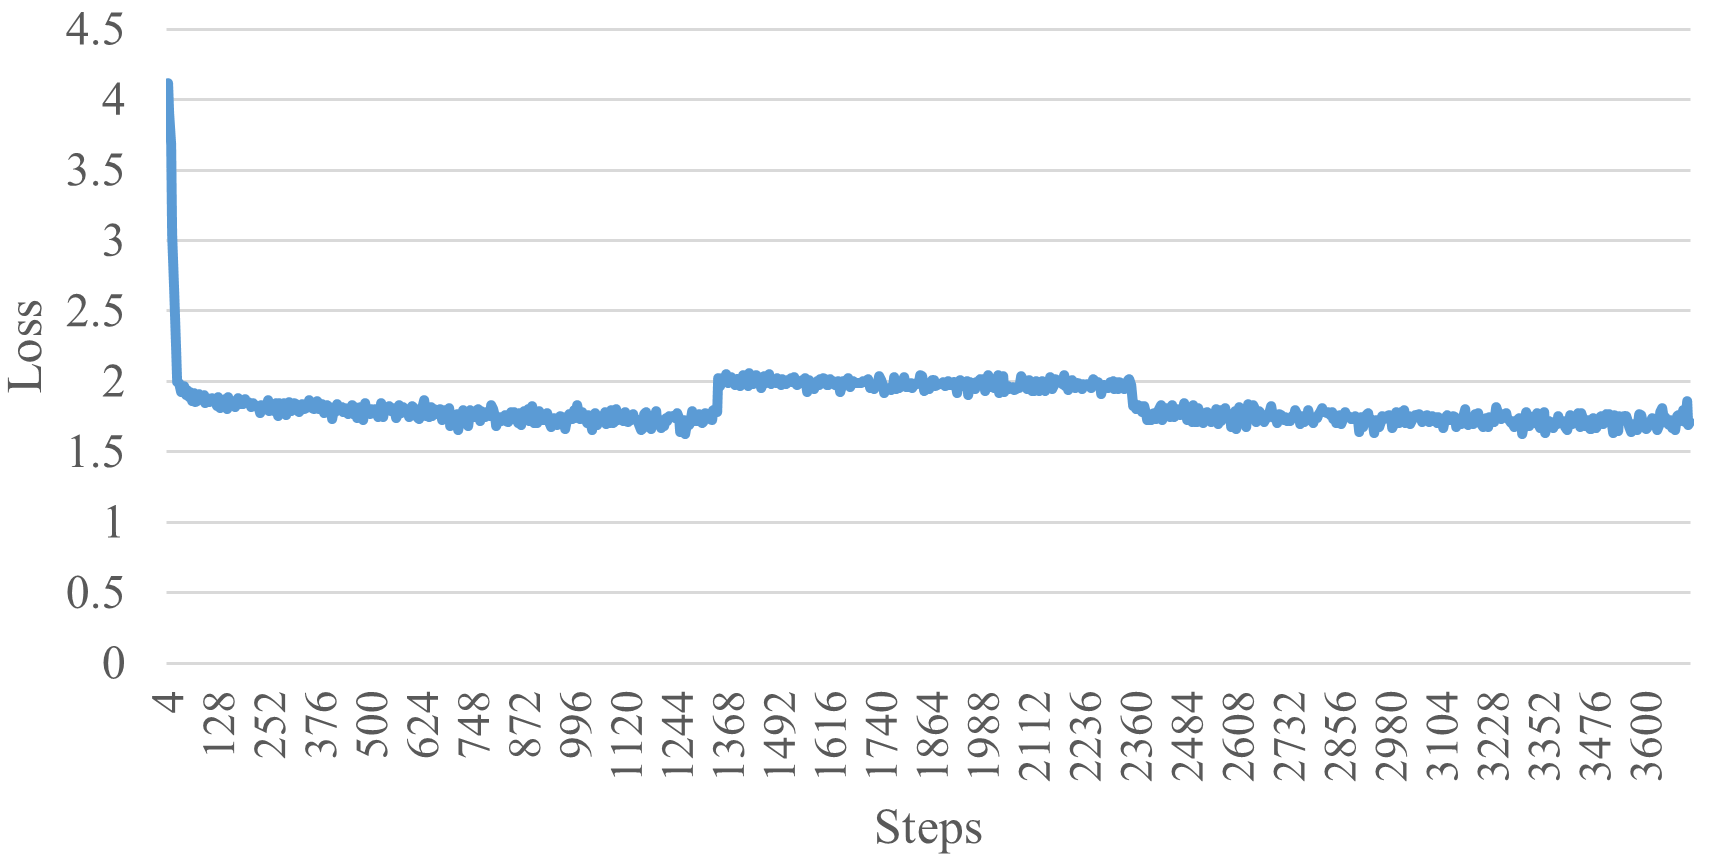
\includegraphics[width=\textwidth]{fig3.png}
\caption{Fine-tuning (domain-adaptation) loss curve}\label{fig3}
\Description{Line plot showing the training loss decreasing over steps during domain adaptation.}
\end{figure}

\begin{figure}[h]
\centering
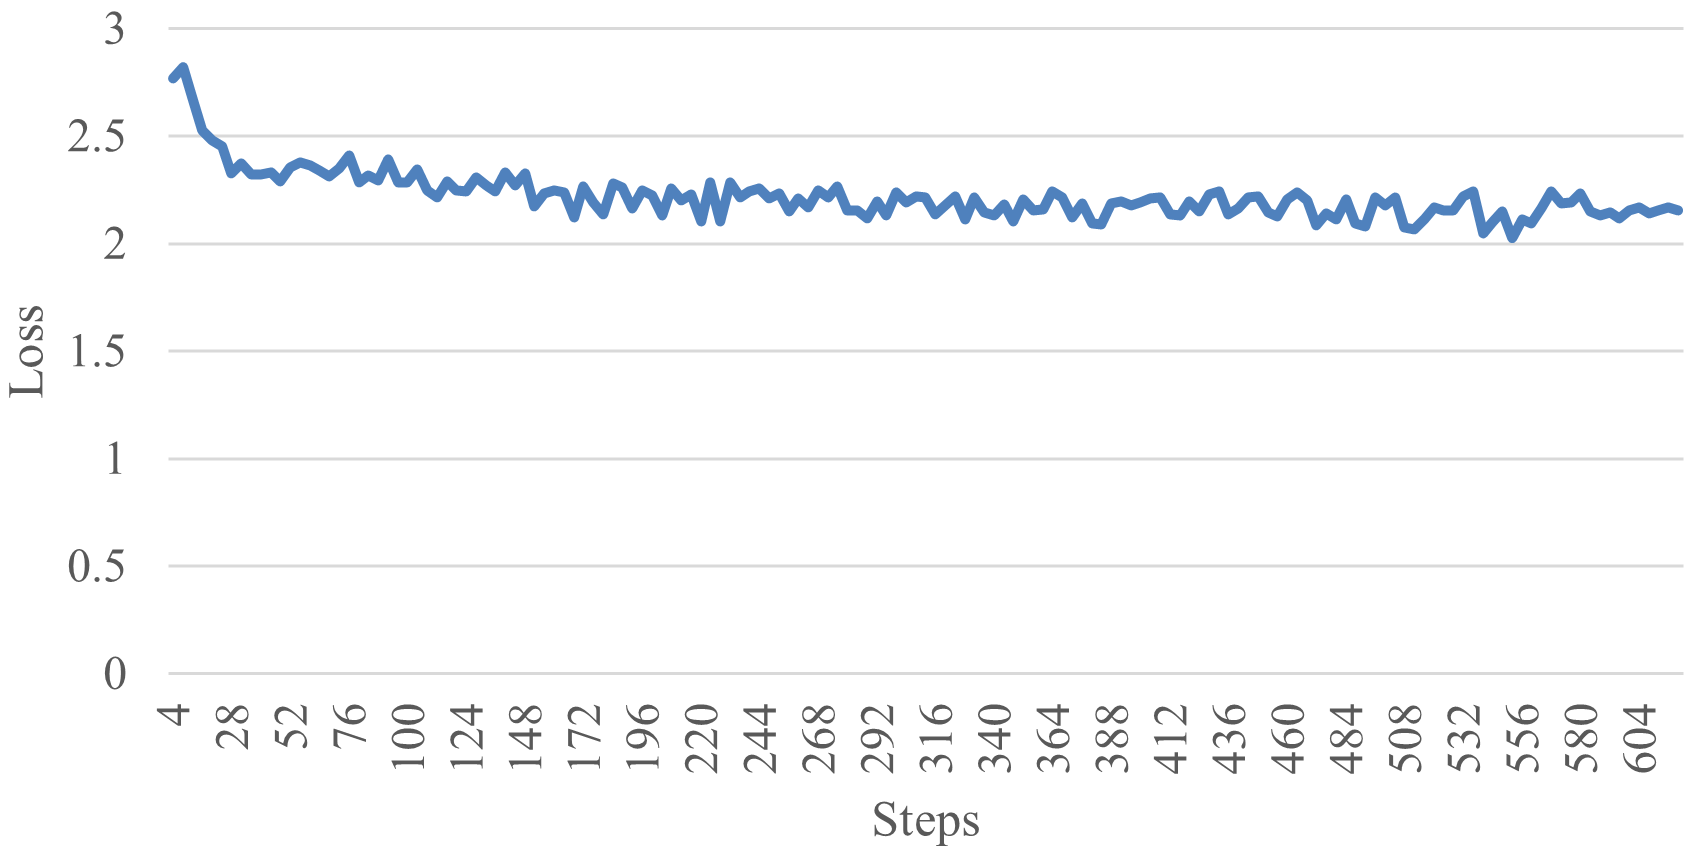
\includegraphics[width=\textwidth]{fig4.png}
\caption{Instruction-tuning loss curve}\label{fig4}
\Description{Line plot showing the training loss decreasing over steps during instruction tuning.}
\end{figure}

\subsection{Gaokerena-R}\label{subsec4.2}

Gaokerena-R is trained with an RLAIF~\cite{b32} pipeline that builds a preference dataset $\mathcal{D}=\{(x,y_w,y_l)\}$, where $x$ is a medical question, $y_w$ a preferred reasoning trajectory and $y_l$ a rejected response, and optimises the student policy $\pi_\theta$ with Direct Preference Optimization (DPO)~\cite{b33} (Eq.~\eqref{fr:DPOloss}; loss in Fig.~\ref{fig5}). The student $\pi_S$ is the baseline Aya-Expanse-8B and the teacher $\pi_T$ is DeepSeek-R1~\cite{b34}. Questions come from the translated MedMCQA training set. Two strategies generate the pairs.

In \textit{Expert-Guided Synthesis}, an incorrect initial student response $y_{\text{init}}$ becomes $y_l$, and the teacher, given the ground-truth answer, writes a correct Chain-of-Thought explanation as $y_w$ (Fig.~\ref{fig6}). In \textit{Iterative Self-Correction}, the teacher instead critiques $y_{\text{init}}$ without revealing the answer; if the student's retry $y_{\text{retry}}$ is correct, it becomes $y_w$ and $y_{\text{init}}$ becomes $y_l$, which keeps preferred trajectories close to the student's own distribution (Fig.~\ref{fig7}). The first strategy dominates: for every 19 pairs it yields, about one comes from the second. The final dataset has about 11,000 pairs (roughly 2 million preferred and 2.5 million rejected tokens).

\begin{equation}
\mathcal{L}_{\text{DPO}} =
-\mathbb{E}_{(x,y_w,y_l)\sim\mathcal{D}}
\left[
\log \sigma\left(
\beta \log\frac{\pi_{\theta}(y_w\mid x)}{\pi_{\text{ref}}(y_w\mid x)}
-\beta \log\frac{\pi_{\theta}(y_l\mid x)}{\pi_{\text{ref}}(y_l\mid x)}
\right)
\right]
\label{fr:DPOloss}
\end{equation}

Here $\sigma$ is the sigmoid function, $\pi_{\text{ref}}$ the reference model and $\beta$ controls the strength of the update relative to it. Minimising $\mathcal{L}_{\text{DPO}}$ raises the probability of $y_w$ relative to $y_l$, which transfers the teacher's reasoning style to Gaokerena-R.

\begin{figure}[h]
\centering
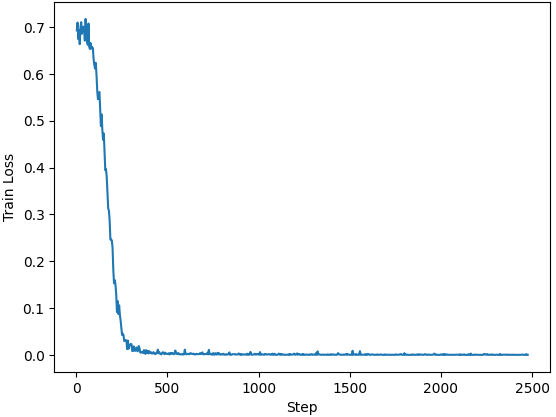
\includegraphics[width=\textwidth]{fig5.png}
\caption{DPO loss curve}\label{fig5}
\Description{Line plot showing the DPO training loss decreasing over steps.}
\end{figure}

\begin{figure}[h]
\centering
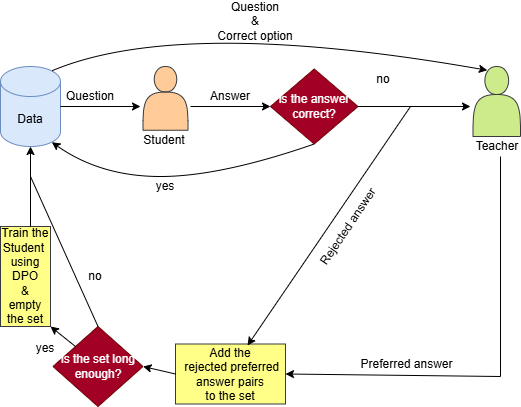
\includegraphics[width=\textwidth]{fig6.png}
\caption{Block diagram of Method 1 (Expert-Guided Synthesis)}\label{fig6}
\Description{Flow diagram showing the Expert-Guided Synthesis pipeline: student generates incorrect response, teacher receives ground-truth answer and produces correct chain-of-thought explanation.}
\end{figure}

\begin{figure}[h]
\centering
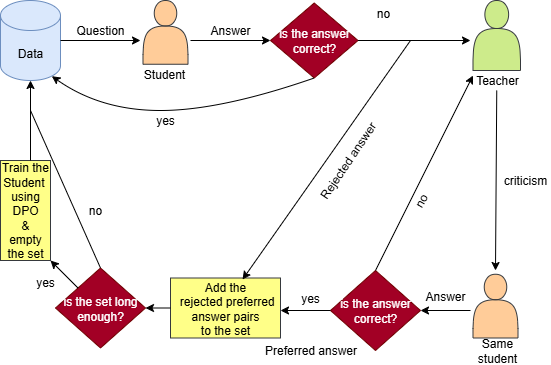
\includegraphics[width=\textwidth]{fig7.png}
\caption{Block diagram of Method 2 (Iterative Self-Correction)}\label{fig7}
\Description{Flow diagram showing the Iterative Self-Correction pipeline: teacher critiques student response without revealing answer, student retries, and correct retry becomes preferred response.}
\end{figure}

%% ------------------------------------------------------------------
\section{Companion Work: Uncertainty Heads}\label{sec:uhead}

Small medical language models can produce fluent but unsupported statements, so we also equip both models with claim-level uncertainty heads. These are lightweight auxiliary modules trained on top of the frozen backbone: from a single forward pass, and using only the backbone's internal signals (attention maps and token probabilities), they estimate whether each generated claim is likely to be supported or hallucinated. They need no external retrieval or repeated sampling and leave the models' generative behaviour unchanged. In a preliminary check on the 168-question KOPP Sept 2023 session, across five generations per question Gaokerena-V produced the same option on only 14 questions and Gaokerena-R on 37, which motivated a claim-level rather than response-level detector. Trained on 1,600 Persian responses per backbone, the heads reach PR-AUCs of 0.4820 and 0.4652 (2.30 and 2.66 times the random baseline) and ROC-AUCs of 0.7852 and 0.7810 on held-out test splits. Dataset construction, architecture, training and full evaluation are reported in~\cite{b3}; the results of this paper do not depend on the heads.

%% ------------------------------------------------------------------
\section{Experiments and Results}\label{sec:results}

Small multilingual models often struggle with under-represented languages such as Persian. Aya-Expanse~\cite{b12,b13} improves Persian fluency, but general-purpose multilingual models still trade off domain performance. This section evaluates our models against general-purpose alternatives on Persian medical MCQs.

\subsection{Setup}\label{subsec6.0}

We report accuracy on the six Persian-translated MMLU medical subsets (FA\_MED\_MMLU, 1,089 questions) and on the KOPP Sept.\ 2023 session (``IBMSEE Sept.\ 2023'', 168 questions). The remaining KOPP sessions are not evaluated here. Baselines are Aya-Expanse-8B (the backbone of both Gaokerena models), Qwen2.5~\cite{b35} (7.6B) and PersianMind~\cite{b14}. All accuracies in the tables are computed from per-question predictions and rounded to two decimals, except those of Table~\ref{tab:cotsc}, which are derived from the per-subject results reported in~\cite{b2}; the MMLU average is pooled over all 1,089 questions, not a mean of subject scores. Results are from a single evaluation run per configuration.

\paragraph{Statistical methods.} Uncertainty from the finite number of test questions is quantified with 95\% Wilson score intervals for each accuracy. Pairwise differences between systems are tested with two-sided two-proportion $z$-tests computed from the number of correct answers. These tests treat the two systems as independent samples; because all systems answer the same questions, a paired test (exact McNemar test on per-question correctness) would normally be more powerful, so the $p$-values reported here should be regarded as conservative approximations. We test the five comparisons per benchmark that correspond to claims made in the text (Table~\ref{tab:significance}) and, separately, the three pairwise comparisons among the matched CoT-SC systems (Table~\ref{tab:cotsc_sig}). These comparisons were chosen after seeing the results, not pre-registered. The tables report uncorrected $p$-values, and the text states where a Holm correction (over the ten tests of Table~\ref{tab:significance}, and over the six matched tests respectively) changes a conclusion. Accuracy against the 36\% pass mark of the entrance exam is tested with a one-sided exact binomial test. We test only pooled accuracy: the per-subject sets (100--272 items) and the 168-item KOPP session are too small to resolve differences of a few points, so per-subject differences in the tables are descriptive. These tests account for sampling variability over test questions only; they do not account for variability across training seeds or across sampling seeds in CoT-SC decoding, which we did not measure. The English--Persian comparisons of Section~\ref{subsec6.3} use the same unpaired tests; Persian counts are recovered from the reported percentages.

\subsection{Gaokerena-V Results}\label{subsec6.1}

Table~\ref{tab:model_results_vs_general_purpose_languages} reports all models under straight (direct, zero-shot) prompting; Gaokerena-R under its preferred CoT-SC strategy is in Section~\ref{subsec6.2}. Confidence intervals and pairwise tests are in Tables~\ref{tab:ci} and~\ref{tab:significance}.

Gaokerena-V has the highest pooled MMLU accuracy among directly prompted models (49.31\%, 537 of 1,089 questions, against 508 for its backbone and 488 for Qwen2.5) and the best score in five of the six subjects; Gaokerena-R under straight prompting is best on college medicine. The margin over the backbone is small, however: +2.66 points with overlapping intervals (46.35--52.28\% against 43.70--49.62\%), and the difference is not statistically significant ($p=0.21$). The difference to Qwen2.5 (+4.50 points) is nominally significant ($p=0.035$) but does not survive a Holm correction over the ten tests. The data are therefore consistent with a modest improvement from domain adaptation and instruction tuning, but do not establish one.

On KOPP Sept.\ 2023, Gaokerena-V scores 38.69\% (65 of 168 questions), above the 36\% pass mark of the Iranian Basic Medical Science Entrance Exam, while all other directly prompted models in Table~\ref{tab:model_results_vs_general_purpose_languages} score below it. This result should be read with care. With 168 questions the 95\% Wilson interval for 38.69\% is 31.66--46.23\%, which includes the pass mark, and the one-sided exact binomial test against 36\% is not significant ($p=0.26$). The difference to Aya-Expanse-8B is seven questions (+4.17 points, $p=0.43$), and a constant-position guess already reaches 32.1\% on this session because of its skewed answer key (Section~\ref{subsubsec:mcq_analysis}). We therefore claim only that the Gaokerena-V point estimate on this single session is above the pass mark, not that the difference is established.

The largest subject gain over the backbone is in anatomy (7.4 percentage points, 10 more correct answers out of 135); with 135 questions this difference is descriptive and untested. Anatomy-focused material may be relatively abundant in reputable Persian digital publications, but we did not test this explanation. Gains in other subjects are smaller; we suspect that the limited volume and uneven quality of Persian medical text restricts further improvement, though we did not test this either.

PersianMind has the lowest inference time, which likely reflects its tendency to give truncated, very short responses. In several subjects its accuracy is close to chance (25.90\% pooled; interval 23.38--28.58\%, which includes the 25\% chance level).

\begin{table}[h]
\caption{Performance of Gaokerena models and general-purpose baselines with straight (direct, zero-shot) prompting (accuracy, \%, single run). Aya-Expanse-8B is the backbone of both Gaokerena models. Subject rows are the Persian-translated MMLU subsets; the MMLU average is pooled over 1,089 questions. Best values in bold. Confidence intervals and significance tests are in Tables~\ref{tab:ci} and~\ref{tab:significance}.}\label{tab:model_results_vs_general_purpose_languages}
\footnotesize
\setlength{\tabcolsep}{3pt}
\begin{tabular}{@{}lccccc@{}}
\toprule
 & Gaokerena-V & Gaokerena-R & Aya-Expanse-8B & Qwen2.5 & PersianMind \\
 & (ours) & (ours) & (backbone) & & \\
\midrule
Anatomy & \textbf{48.15} & 41.48 & 40.74 & 41.48 & 25.19 \\
Medical genetics & \textbf{53.00} & 49.00 & 49.00 & 52.00 & 34.00 \\
College medicine & 43.93 & \textbf{46.24} & 44.51 & 43.35 & 20.23 \\
Clinical knowledge & \textbf{55.47} & 52.45 & 52.08 & 47.92 & 25.28 \\
Professional medicine & \textbf{47.06} & 41.91 & 45.59 & 43.01 & 23.90 \\
College biology & \textbf{47.22} & 44.44 & 45.14 & 42.36 & 32.64 \\
MMLU avg.\ (pooled) & \textbf{49.31} & 46.10 & 46.65 & 44.81 & 25.90 \\
IBMSEE Sept.\ 2023 & \textbf{38.69} & 35.12 & 34.52 & 33.33 & 19.64 \\
\midrule
Parameters & 8B & 8B & 8B & 7.6B & 6.8B \\
Prompt type & Straight & Straight & Straight & Straight & Straight \\
Inference time & $\approx$10 s & $\approx$10 s & $\approx$10 s & $\approx$15 s & $\approx$2 s \\
\bottomrule
\end{tabular}
\end{table}

\begin{table}[h]
\caption{Pooled accuracy with 95\% Wilson confidence intervals (\%). Gaokerena-R is shown under both straight prompting and its preferred CoT-SC configuration (not compute-matched to the direct baselines). MMLU: $n=1{,}089$; KOPP Sept.\ 2023: $n=168$.}\label{tab:ci}
\small
\begin{tabular}{@{}lcc@{}}
\toprule
System & MMLU pooled (95\% CI) & KOPP Sept.\ 2023 (95\% CI) \\
\midrule
Gaokerena-V (direct) & 49.31 [46.35, 52.28] & 38.69 [31.66, 46.23] \\
Gaokerena-R (direct) & 46.10 [43.16, 49.07] & 35.12 [28.31, 42.60] \\
Gaokerena-R (CoT-SC) & 52.80 [49.83, 55.75] & 46.43 [39.05, 53.97] \\
Aya-Expanse-8B (direct) & 46.65 [43.70, 49.62] & 34.52 [27.75, 41.99] \\
Qwen2.5 (direct) & 44.81 [41.88, 47.78] & 33.33 [26.65, 40.76] \\
PersianMind (direct) & 25.90 [23.38, 28.58] & 19.64 [14.34, 26.30] \\
\bottomrule
\end{tabular}
\end{table}

\begin{table}[h]
\caption{Pairwise comparisons of accuracy: difference in percentage points (first system minus second) and two-sided $p$-value from an unpaired two-proportion $z$-test. $p$-values are uncorrected; after Holm correction over all ten tests only the starred comparison (MMLU, Gaokerena-R CoT-SC vs.\ Aya-Expanse-8B) remains significant at 0.05. Paired McNemar tests on per-question correctness would normally be more powerful.}\label{tab:significance}
\small
\begin{tabular}{@{}lrrrr@{}}
\toprule
 & \multicolumn{2}{c}{MMLU pooled} & \multicolumn{2}{c}{KOPP Sept.\ 2023} \\
\cmidrule(lr){2-3}\cmidrule(lr){4-5}
Comparison & $\Delta$ & $p$ & $\Delta$ & $p$ \\
\midrule
Gaokerena-V vs.\ Aya-Expanse-8B (direct) & $+2.66$ & 0.21 & $+4.17$ & 0.43 \\
Gaokerena-V vs.\ Qwen2.5 (direct) & $+4.50$ & 0.035 & $+5.36$ & 0.31 \\
Gaokerena-R (CoT-SC) vs.\ Gaokerena-V (direct) & $+3.49$ & 0.10 & $+7.74$ & 0.15 \\
Gaokerena-R (CoT-SC) vs.\ Aya-Expanse-8B (direct) & $+6.15$ & 0.004$^{*}$ & $+11.90$ & 0.026 \\
Gaokerena-R (direct) vs.\ Aya-Expanse-8B (direct) & $-0.55$ & 0.80 & $+0.60$ & 0.91 \\
\bottomrule
\end{tabular}
\end{table}

\subsection{Gaokerena-R Results}\label{subsec6.2}

Gaokerena-R is designed to use structured reasoning, so we evaluate it under chain-of-thought (CoT) prompting as well as direct prompting. Under straight prompting it does not outperform its backbone (46.10\% against 46.65\% pooled; $p=0.80$; Table~\ref{tab:model_results_vs_general_purpose_languages}), so the system prompt must instruct it to reason step by step.

\paragraph{Matched CoT self-consistency.} We first compare the three models under identical conditions (Table~\ref{tab:cotsc}). Each model receives a CoT prompt and generates five responses per question at temperature 1.0, and a self-consistency rule~\cite{b36} accepts an answer only when at least three of the five responses choose the same option; otherwise the question is left unanswered and counted as incorrect. All three models therefore receive the same inference computation, and no verifier is used. Gaokerena-R reaches 48.67\% pooled MMLU accuracy against 46.92\% for the backbone ($+1.75$ points, $p=0.41$) and 40.13\% for Gaokerena-V. The difference to Gaokerena-V ($+8.54$ points, $p<0.001$) is significant, but the difference to the backbone is not significant on MMLU or on KOPP (38.69\% against 35.71\%, $p=0.57$). In this setting Gaokerena-V scores significantly below its own backbone ($-6.80$ points, $p=0.001$): domain adaptation and instruction tuning do not help, and appear to hurt, CoT self-consistency accuracy. Because unanswered questions count as errors, this may partly reflect more abstentions rather than more wrong answers, and we did not record coverage separately. Under matched computation, the data therefore do not establish that DPO improves on the backbone; they do show that Gaokerena-R is far better than Gaokerena-V when both are asked to reason.

\paragraph{Adding a verifier.} Gaokerena-R's preferred configuration resolves questions without a three-vote majority by asking Aya-Expanse-8B, the backbone, to act as an external verifier on the conflicting responses. This raises pooled MMLU accuracy from 48.67\% to 52.80\% (575 of 1,089 questions, 45 more correct answers), and KOPP Sept.\ 2023 accuracy to 46.43\%, at roughly 19 times the per-question inference time of the direct baselines (about 193 s against about 10 s; Table~\ref{tab:med_opns_comparison}). Compared with the directly prompted systems of Table~\ref{tab:med_opns_comparison}, Gaokerena-R is 3.49 points above Gaokerena-V and 6.15 points above Aya-Expanse-8B. The difference to Aya-Expanse-8B is significant on pooled MMLU ($p=0.004$, which survives Holm correction) and nominally on KOPP ($p=0.026$, which does not survive correction over ten tests); the difference to Gaokerena-V is not significant on either benchmark ($p=0.10$ and $p=0.15$). On KOPP, the interval for Gaokerena-R (39.05--53.97\%) lies above the 36\% pass mark (one-sided exact binomial $p=0.003$), in contrast to Gaokerena-V.

This comparison is not compute-matched: CoT prompting, five samples and a verifier give Gaokerena-R substantially more inference computation than the directly prompted baselines, so Table~\ref{tab:med_opns_comparison} shows the best configuration of each model, not the effect of DPO alone. The missing control is the backbone run through the identical CoT-SC-plus-verifier pipeline; we did not run it, so we cannot say how much of the 6.15-point gain comes from training and how much from test-time computation and the verifier, which is itself the backbone.

\paragraph{Why direct and CoT results differ.} The three models respond very differently to the change from direct prompting to CoT self-consistency. Pooled MMLU accuracy moves from 46.10\% to 48.67\% for Gaokerena-R ($+2.6$ points), from 46.65\% to 46.92\% for the backbone ($+0.3$) and from 49.31\% to 40.13\% for Gaokerena-V ($-9.2$ points; $p<0.001$, unpaired). We did not design experiments to explain this, and the two settings differ in more than prompt format (a single response against five samples at temperature 1.0, and a rule that counts unanswered questions as errors), so we offer hypotheses, not conclusions. (i)~\emph{Format match.} The preferred responses used to train Gaokerena-R are teacher-written chain-of-thought explanations, so step-by-step output is within its training distribution, whereas Gaokerena-V was adapted on corpus text and on MF3QA answers, which are direct, free-form replies rather than explicit reasoning; long reasoning chains may lie further from what it was trained to produce. (ii)~\emph{Sampling instability.} Gaokerena-V's answers vary widely between samples (Section~\ref{sec:uhead}: across five generations on KOPP Sept.\ 2023, all five picked the same option for only 14 of 168 questions, against 37 for Gaokerena-R), so it fails the three-vote rule more often, and every failure counts as an error; at temperature 1.0, long chains also compound small sampling deviations. (iii)~\emph{Additional failure modes.} Direct prompting tests whether the correct option is the model's immediate preference, whereas CoT adds ways to fail, since an early incorrect or unsupported step can steer the final answer away from a correct recall. (iv)~\emph{Output problems.} We did not measure how often CoT outputs lacked a parsable final option or drifted into another language, either of which would lower CoT accuracy. We therefore do not conclude that training on raw corpora damages reasoning, only that Gaokerena-V scores lower under this CoT-SC protocol. Separating these explanations would require reporting coverage and per-sample accuracy under CoT, answer-extraction failure rates, and direct prompting and CoT at matched temperature (or greedy decoding).

\begin{table}[h]
\caption{Matched comparison: CoT prompting, five samples at temperature 1.0 and a three-vote majority, without a verifier (accuracy, \%, single run). Questions without a majority are unanswered and counted as incorrect. Values are the per-subject results reported in~\cite{b2}, converted to counts and pooled by us (MMLU: $n=1{,}089$; KOPP Sept.\ 2023: $n=168$); the pooled averages therefore differ slightly from those printed in~\cite{b2}. Best values in bold.}\label{tab:cotsc}
\small
\begin{tabular}{@{}lccc@{}}
\toprule
 & Gaokerena-R & Gaokerena-V & Aya-Expanse-8B \\
\midrule
Anatomy & \textbf{42.22} & 39.26 & 40.74 \\
Medical genetics & \textbf{50.00} & 41.00 & 45.00 \\
College medicine & 47.98 & 37.57 & \textbf{48.55} \\
Clinical knowledge & \textbf{55.85} & 46.79 & 54.72 \\
Professional medicine & \textbf{44.85} & 37.13 & 43.75 \\
College biology & \textbf{48.61} & 36.81 & 43.75 \\
MMLU avg.\ (pooled) & \textbf{48.67} & 40.13 & 46.92 \\
\quad 95\% CI & [45.71, 51.64] & [37.26, 43.07] & [43.98, 49.89] \\
IBMSEE Sept.\ 2023 & \textbf{38.69} & 29.76 & 35.71 \\
\quad 95\% CI & [31.66, 46.23] & [23.36, 37.07] & [28.86, 43.21] \\
\midrule
Prompt & CoT & CoT & CoT \\
Decoding & CoT-SC (no verifier) & CoT-SC (no verifier) & CoT-SC (no verifier) \\
Generation time & $\approx 5\times 35$ s & $\approx 5\times 35$ s & $\approx 5\times 35$ s \\
\bottomrule
\end{tabular}
\end{table}

\begin{table}[h]
\caption{Pairwise comparisons among the matched CoT-SC systems of Table~\ref{tab:cotsc}: difference in percentage points (first system minus second) and two-sided $p$-value from an unpaired two-proportion $z$-test (uncorrected). After Holm correction over these six tests, the two MMLU comparisons with Gaokerena-V remain significant at 0.05; the others do not.}\label{tab:cotsc_sig}
\small
\begin{tabular}{@{}lrrrr@{}}
\toprule
 & \multicolumn{2}{c}{MMLU pooled} & \multicolumn{2}{c}{KOPP Sept.\ 2023} \\
\cmidrule(lr){2-3}\cmidrule(lr){4-5}
Comparison & $\Delta$ & $p$ & $\Delta$ & $p$ \\
\midrule
Gaokerena-R vs.\ Aya-Expanse-8B & $+1.75$ & 0.41 & $+2.98$ & 0.57 \\
Gaokerena-R vs.\ Gaokerena-V & $+8.54$ & $<$0.001 & $+8.93$ & 0.085 \\
Aya-Expanse-8B vs.\ Gaokerena-V & $+6.80$ & 0.001 & $+5.95$ & 0.25 \\
\bottomrule
\end{tabular}
\end{table}

\begin{table}[h]
\caption{Performance of Gaokerena models with the preferred prompting strategy of each model (accuracy, \%, single run). The configurations are not compute-matched; the matched comparison is in Table~\ref{tab:cotsc}. Subject rows are the Persian-translated MMLU subsets; the MMLU average is pooled over 1,089 questions. Best values in bold. Confidence intervals and significance tests are in Tables~\ref{tab:ci} and~\ref{tab:significance}.}\label{tab:med_opns_comparison}
\small
\begin{tabular*}{\textwidth}{@{\extracolsep\fill}lccc}
\toprule
 & Gaokerena-R & Gaokerena-V & Aya-Expanse-8B \\
\midrule
Anatomy & 47.41 & \textbf{48.15} & 40.74 \\
Medical genetics & \textbf{56.00} & 53.00 & 49.00 \\
College medicine & \textbf{50.29} & 43.93 & 44.51 \\
Clinical knowledge & \textbf{58.87} & 55.47 & 52.08 \\
Professional medicine & \textbf{48.90} & 47.06 & 45.59 \\
College biology & \textbf{54.86} & 47.22 & 45.14 \\
MMLU avg.\ (pooled) & \textbf{52.80} & 49.31 & 46.65 \\
IBMSEE Sept.\ 2023 & \textbf{46.43} & 38.69 & 34.52 \\
\midrule
Prompt & CoT & Direct & Direct \\
Decoding & CoT-SC (with verifier) & Zero-shot & Zero-shot \\
Inference time & $\approx 5\times 35+10+8$ s & $\approx$10 s & $\approx$10 s \\
\bottomrule
\end{tabular*}
\end{table}

Because Gaokerena-R is sampled several times per question, we also use the \emph{pass@k} metric of Brown et al.~\cite{b37}, the probability that at least one of $k$ sampled answers is correct (Eq.~\eqref{fr:passatk}), where $M=5$ is the number of samples per question and $C$ the number of correct samples. We report the average pass@k for $k\leq 3$ over the full test set. Higher $k$ is omitted because with four options a model that selects every option would trivially reach 100\% at $k=4$. As Figs.~\ref{fig8} and~\ref{fig9} show, the Gaokerena-R curve lies above those of Gaokerena-V and the Aya-Expanse-8B baseline in nearly all categories, with anatomy the exception, where Gaokerena-V is slightly better. We read this as evidence that Gaokerena-R's correct answers are more often among its first few samples. All three models were sampled under identical CoT prompting (five samples, temperature 1.0, no verifier), so unlike Table~\ref{tab:med_opns_comparison} this comparison is matched in computation. We did not test the pass@k differences for significance, so the curves should be read together with the tests of Table~\ref{tab:cotsc_sig}, which find no significant gap to the backbone. We do not interpret the curves as evidence of calibrated confidence, which we did not measure. The high response variability we observed for Gaokerena-V (Section~\ref{sec:uhead}) may inflate its pass@k at larger $k$, where random guessing is more effective, but we did not test this.

\begin{equation}
\text{pass@k} = 1 - \frac{\binom{M-C}{k}}{\binom{M}{k}}
\label{fr:passatk}
\end{equation}

\begin{figure}[h]
\centering
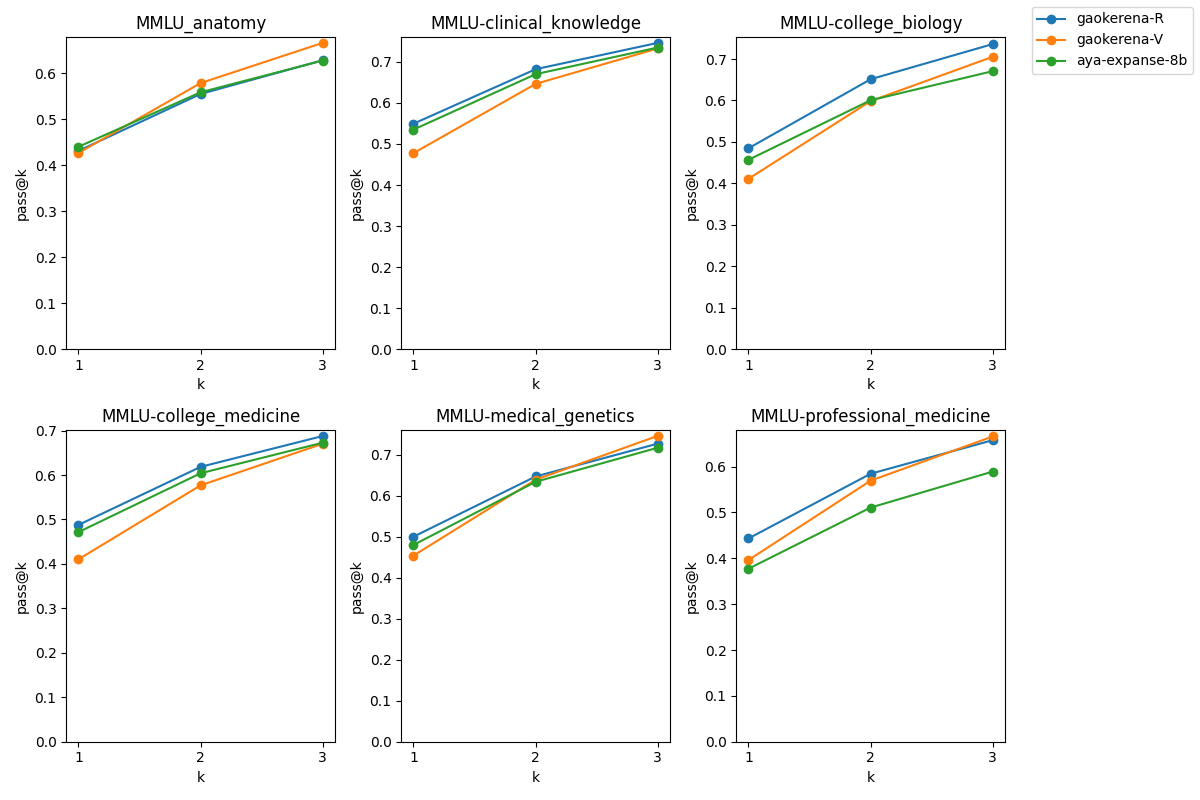
\includegraphics[width=\textwidth]{fig8.png}
\caption{Pass@k results on the Persian-translated medical portion of the MMLU dataset}\label{fig8}
\Description{Line plot showing pass@k scores for Gaokerena-R, Gaokerena-V, and Aya-Expanse-8B across k values 1 to 3 on the translated MMLU medical subset.}
\end{figure}

\begin{figure}[h]
\centering
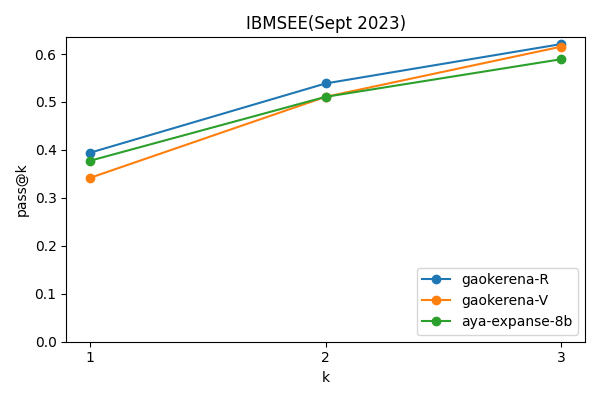
\includegraphics[width=0.8\textwidth]{fig9.png}
\caption{Pass@k results on the IBMSEE Sept.\ 2023 dataset}\label{fig9}
\Description{Line plot showing pass@k scores for Gaokerena-R, Gaokerena-V, and Aya-Expanse-8B across k values 1 to 3 on the IBMSEE Sept 2023 dataset.}
\end{figure}

%% ------------------------------------------------------------------
\subsection{English--Persian Gap}\label{subsec6.3}

The Persian MMLU medical subsets are translations of the English test partitions (Section~\ref{subsubsec:mcq_analysis}), so the same questions can be put to the backbone in English. This gives a direct reference for how much is lost when the language changes. We ran Aya-Expanse-8B on the original English questions of the six subjects (1,089 questions) under the two protocols used for Persian: straight prompting, and CoT prompting with five experiments and the three-vote self-consistency rule of Section~\ref{subsec6.2} (no verifier; questions without a three-vote majority count as incorrect). The English prompts are a direct translation of the Persian prompts, with the instruction to answer in English. Where an English experiment file contains more than one generation per question, we used the first one, so each English CoT-SC result is computed from five generations per question. Accuracies are pooled over all 1,089 questions, as in the Persian tables.

\paragraph{Results.} Table~\ref{tab:en_fa} shows that the model answers the same questions much more accurately in English. Under straight prompting, Aya-Expanse-8B reaches 59.04\% in English (643 of 1,089; 95\% Wilson interval 56.10--61.93\%) against 46.65\% in Persian, a gap of 12.40 points ($p<0.001$, unpaired two-proportion $z$-test). Under CoT-SC the English accuracy is 63.18\% (688 of 1,089; interval 60.27--65.99\%; 88.9\% of questions reach a three-vote majority), against 46.92\% in Persian, a gap of 16.25 points ($p<0.001$). CoT-SC raises English accuracy by 4.13 points over straight prompting ($p=0.048$, unpaired), whereas it leaves the Persian backbone unchanged ($+0.27$ points), so the gap is larger when the model is asked to reason.

\begin{table}[h]
\caption{Pooled accuracy (\%) on the six medical MMLU subjects (1,089 questions) in English and Persian, single runs. For each Persian system, $\Delta$ is English Aya-Expanse-8B minus that system (percentage points) and $p$ is from an unpaired two-proportion $z$-test (uncorrected); the English row has no counterpart and is left blank. The verifier configuration has no English counterpart, so its two $\Delta$/$p$ entries compare it against English straight prompting and English CoT-SC, respectively. Persian counts are recovered from the percentages of Tables~\ref{tab:model_results_vs_general_purpose_languages} and~\ref{tab:cotsc}.}\label{tab:en_fa}
\small
\setlength{\tabcolsep}{4pt}
\begin{tabular}{@{}llccc@{}}
\toprule
Prompting & Model & Accuracy & $\Delta$ vs.\ English & $p$ \\
\midrule
Straight & English Aya-Expanse-8B & 59.04 & --- & --- \\
         & Persian Aya-Expanse-8B & 46.65 & $+12.40$ & $<$0.001 \\
         & Persian Gaokerena-V    & 49.31 & $+9.73$  & $<$0.001 \\
         & Persian Gaokerena-R    & 46.10 & $+12.95$ & $<$0.001 \\
\midrule
CoT-SC, no verifier & English Aya-Expanse-8B & 63.18 & --- & --- \\
                    & Persian Aya-Expanse-8B & 46.92 & $+16.25$ & $<$0.001 \\
                    & Persian Gaokerena-V    & 40.13 & $+23.05$ & $<$0.001 \\
                    & Persian Gaokerena-R    & 48.67 & $+14.51$ & $<$0.001 \\
\midrule
CoT-SC + verifier & Persian Gaokerena-R & 52.80 & $+6.24$ / $+10.38$ & 0.003 / $<$0.001 \\
\bottomrule
\end{tabular}
\end{table}

\paragraph{How much of the gap the Persian resources close.} Relative to the English reference, Gaokerena-V under straight prompting narrows the gap from 12.40 to 9.73 points, and Gaokerena-R with CoT-SC and the verifier (52.80\%) is 6.24 points below English straight prompting and 10.38 below English CoT-SC. These are the largest reductions in the gap that we observe, but they should be read with the caveats of Sections~\ref{subsec6.1} and~\ref{subsec6.2}. The Gaokerena-V improvement over the backbone is not significant ($p=0.21$); the Gaokerena-R configuration uses several times the inference computation of the straight-prompted English model and the backbone was never run through the same verifier pipeline; and under matched CoT-SC without the verifier the gap is 14.51 points for Gaokerena-R against 16.25 for the backbone, a narrowing of 1.75 points that is not significant ($p=0.41$, Section~\ref{subsec6.2}). Gaokerena-V widens the gap under CoT-SC (23.05 points). In every configuration the Persian systems remain significantly below the English backbone.

\paragraph{By subject.} Table~\ref{tab:en_fa_subject} gives the straight-prompting results per subject. The gap is uneven: it is largest in college biology (27.08 points for the backbone) and anatomy (18.52), and almost absent in professional medicine (2.20), where English straight-prompting accuracy is itself the lowest of the six subjects. Gaokerena-V reduces the gap most in anatomy (to 11.11 points), the subject with its largest gain over the backbone, and in clinical knowledge (from 13.20 to 9.81). With 100--272 questions per subject these differences are descriptive and are not tested.

\begin{table}[h]
\caption{Straight-prompting accuracy (\%) per subject, English against Persian. Gap columns are English Aya-Expanse-8B minus the Persian system (percentage points). Descriptive; single runs.}\label{tab:en_fa_subject}
\small
\begin{tabular}{@{}lrrrrr@{}}
\toprule
Subject & $n$ & English Aya & Persian Aya & Persian Gaokerena-V & Gap (Aya / V) \\
\midrule
Anatomy & 135 & 59.26 & 40.74 & 48.15 & 18.52 / 11.11 \\
Medical genetics & 100 & 64.00 & 49.00 & 53.00 & 15.00 / 11.00 \\
College medicine & 173 & 53.18 & 44.51 & 43.93 & 8.67 / 9.25 \\
Clinical knowledge & 265 & 65.28 & 52.08 & 55.47 & 13.20 / 9.81 \\
Professional medicine & 272 & 47.79 & 45.59 & 47.06 & 2.20 / 0.73 \\
College biology & 144 & 72.22 & 45.14 & 47.22 & 27.08 / 25.00 \\
\midrule
Pooled & 1,089 & 59.04 & 46.65 & 49.31 & 12.40 / 9.73 \\
\bottomrule
\end{tabular}
\end{table}

\paragraph{Interpretation and caveats.} The results show a large and statistically clear gap between English and Persian for the same questions and the same 8B model. Our working explanation is that it reflects the much smaller amount of Persian medical text available to the model: Persian medical resources were scarce at the start of this work (Section~\ref{sec1}), and the data, reasoning distillation and test-time computation we add recover only part of what is lost, at the price of substantially higher inference cost for the best configuration. We stress that this explanation is a hypothesis; our experiments were not designed to isolate its cause, and the following factors are confounded with it. (i)~\emph{Contamination.} MMLU is public and in English, so the English questions may be better represented in the pretraining or post-training data of Aya-Expanse than their translations; we did not test this. (ii)~\emph{Translation.} The Persian items are translations with the artefacts described in Section~\ref{subsubsec:mcq_analysis}, which can lower accuracy independently of model ability. (iii)~\emph{General Persian proficiency.} Part of the gap may reflect weaker Persian language understanding, tokenisation efficiency or answer-format following in general, not missing medical knowledge. (iv)~\emph{Protocol.} Prompts, decoding and answer extraction were not identical across the two languages, and the English runs are a single evaluation with first-generation selection. (v)~\emph{Statistics.} The tests are unpaired and conservative for same-question comparisons, with Persian counts reconstructed from rounded percentages, and, as before, only variability over test questions is quantified.

We therefore conclude that a substantial English--Persian gap exists in this setting, that our resources, reasoning training and self-consistency narrow it in point estimate but do not close it, and that the evidence that the narrowing comes from the training methods, as opposed to additional inference computation, is suggestive rather than conclusive. Establishing the role of Persian data scarcity would need further experiments: running the backbone and Gaokerena models through identical protocols in both languages, paired per-question analysis, repeated runs across seeds, controls for contamination and for translation quality (for example, a back-translated or re-annotated subset), and training-data scaling experiments.

\paragraph{Why not translate?} The English--Persian gap raises the obvious alternative of translating Persian questions into English, answering them with an English medical model and translating the answer back. We did not evaluate this alternative here, and stronger translators than the small on-device ones tried in~\cite{b1}, which performed poorly, may make it competitive. Even so, there are reasons to develop models that work directly in Persian. A single local model avoids the memory and latency cost of a multi-model pipeline and the translation errors that such a pipeline compounds on medical terminology. It also keeps patient data on the device without relying on external translation services, and it does not leave Persian-speaking communities dependent on resources built for another language. Our results suggest that part of the gap can be narrowed with modest, self-funded resources (about 19 GPU-hours on one A100 for Gaokerena-V~\cite{b1} and about one GPU-hour on one H100 for the DPO stage of Gaokerena-R, excluding data generation~\cite{b2}), but they do not show that it can be closed: the Persian systems remain significantly below the English backbone in every configuration, and the evidence that training, rather than extra inference computation, drives the narrowing is suggestive rather than conclusive. We therefore present direct Persian models as a direction worth pursuing for access and equity, not as a demonstrated replacement for translation.

%% ------------------------------------------------------------------
\section{Limitations}\label{sec:limitations}

\begin{itemize}

\item \textbf{Evaluation scope.} Results are single runs. We report confidence intervals and unpaired significance tests, which capture sampling variability over test questions but not variability across training or decoding seeds, and the unpaired tests are conservative relative to paired tests. Several pairwise comparisons are not significant (notably Gaokerena-V against its backbone), and none of the KOPP differences survive correction for multiple comparisons. The KOPP evaluation uses one 168-question session, and the MMLU evaluation is dominated by two subjects. The headline Gaokerena-R configuration (CoT-SC with verifier) is not compute-matched to the direct baselines, and the backbone has not been run through the same CoT-SC-plus-verifier pipeline; the matched comparison without verifier shows no significant gain over the backbone (Section~\ref{subsec6.2}), and its pooled accuracies are derived from subject-level results and record unanswered questions as errors without reporting coverage. We provide no ablations of the domain-adaptation and instruction-tuning stages or of the two distillation strategies.

\item \textbf{English--Persian comparison.} The comparison does not separate Persian data scarcity from contamination of the English public benchmark, translation artefacts, general Persian proficiency and protocol differences, and the English runs were evaluated only once.

\item \textbf{MF3QA is not evaluated.} We do not report free-form evaluation of Gaokerena-V on MF3QA (automatic metrics, LLM-judge or expert review). Overlap with the corpus makes the development split unsuitable for this purpose (Section~\ref{subsubsec:mf3qa_analysis}). The GPT-4o preference evaluation in the conference version~\cite{b1} is not repeated because we found GPT-4o unreliable as a judge of Persian medical text, and no validated judge or expert review is available.

\item \textbf{Contamination.} We checked overlap between MF3QA and the corpus, and duplication among the benchmarks, but not overlap between the training sources (the corpus, translated MedMCQA, the DPO data) and the evaluation sets.

\item \textbf{Benchmark quality.} KOPP contains PDF-extraction artefacts and answer-key skew, and FA\_MED\_MMLU inherits English annotation errors and was not audited by back-translation or a second annotator. The MCQ format itself is a limited proxy for clinical competence.

\item \textbf{Training data.} The corpus includes loosely medical and syndicated content, and MF3QA contains repeated answers, some recommending unsupported home procedures, and has no safety-specific filtering. The models inherit these properties.

\item \textbf{Baselines.} The baselines are limited to three general-purpose models of similar size. We did not compare with other recent multilingual small models or with larger models.

\item \textbf{Intended use.} Gaokerena-V and Gaokerena-R are research artefacts and are not cleared for clinical use. They should not be used for medical advice, in particular for dosing.

\end{itemize}

%% ------------------------------------------------------------------
\section{Ethical Considerations}\label{sec:ethics}

This study involved no direct interaction with human participants. The corpus, MF3QA and the other text resources were collected from publicly accessible Persian medical websites and forums; no private or access-restricted data were collected. Beyond the personal-data removal applied during cleaning (Section~\ref{subsec3.2}), we applied no additional anonymisation: the text is distributed as it appeared on the public pages. Section~\ref{subsubsec:mf3qa_analysis} quantifies the residual personal data in MF3QA: at most 18 of the 24,000 cleaned pairs contain a phone number, e-mail address, URL or social-media handle, and named physicians and sensitive health topics (including questions from self-identified minors) occur in the text.

We recommend that users of MF3QA apply the filtering and masking steps in Section~\ref{subsubsec:mf3qa_analysis} before any redistribution.

%% ------------------------------------------------------------------
\section{Conclusion}\label{sec:conclusion}

We released an open suite of Persian medical resources, namely a corpus, a patient--doctor QA dataset, a medical MCQ benchmark and a translated MCQ training set, together with detailed characterisations that document their composition, selection effects and limitations. We also released two small models built on them. On translated medical MMLU, Gaokerena-V is 2.66 percentage points above its Aya-Expanse-8B backbone under direct prompting, a difference that is not statistically significant ($p=0.21$), while Gaokerena-R reaches 52.80\% with CoT-SC and a verifier, significantly above the directly prompted backbone ($p=0.004$) but not significantly above Gaokerena-V ($p=0.10$). Under matched CoT self-consistency without the verifier, Gaokerena-R is clearly above Gaokerena-V (48.7\% against 40.1\%) but not significantly above the backbone (46.9\%, $p=0.41$), and Gaokerena-V scores below the backbone. Run on the same questions in English, the backbone is 12--16 points more accurate than in Persian, so a substantial gap remains that our resources and methods only partly narrow. Because these comparisons are single-run and use unpaired tests, and the headline configuration is not compute-matched, the evidence for the training methods is suggestive rather than conclusive. Future work includes paired tests and repeated runs across seeds, running the backbone through the full CoT-SC-plus-verifier pipeline, ablations, free-form evaluation on MF3QA, an audit of the translated benchmark, stronger baselines, and expert evaluation of safety.

%% ------------------------------------------------------------------
\section*{Data and Code Availability}

The medical corpus, MF3QA (and its uncleaned crawl), the benchmarks (KOPP and FA\_MED\_MMLU) and the translated MedMCQA training set are available at \url{https://huggingface.co/datasets/gaokerena} (the translated MedMCQA set is in the Gaokerena-R repository). Code, model weights and generated model responses are available at \url{https://github.com/Mehrdadghassabi/Gaokerena-V} and \url{https://github.com/Mehrdadghassabi/Gaokerena-R}.

\section*{Author Contributions}

M.G. led and carried out all aspects of the work. H.B.K. supervised the research. Z.K. and M.T. were responsible for data collection. A.P. was responsible for translation. P.R., S.H. and A.E. contributed to technical aspects of the work. All authors read and approved the final manuscript.

\section*{Competing Interests}

The authors declare no competing interests.

\begin{acks}
This research received no external funding and was self-funded by the authors.
\end{acks}

%% ------------------------------------------------------------------
\begin{thebibliography}{00}

\bibitem{b1}
Ghassabi, Mehrdad, et al. ``Leveraging online data to enhance medical knowledge in a small persian language model.'' 2025 32nd National and 10th International Iranian Conference on Biomedical Engineering (ICBME). IEEE, 2025.

\bibitem{b2}
Ghassabi, Mehrdad, et al. ``Enhancing Reasoning Skills in Small Persian Medical Language Models Can Outperform Large-Scale Data Training.'' 2025 11th International Conference on Signal Processing and Intelligent Systems (ICSPIS). IEEE, 2025.

\bibitem{b3}
Ghassabi, Mehrdad, et al. ``Single-Pass Uncertainty Heads for Claim-Level Hallucination Detection in Persian Medical Language Models.'' arXiv preprint arXiv:2610.03482 (2026).

\bibitem{b4}
Vaswani, Ashish, et al. ``Attention is all you need.'' Advances in neural information processing systems 30 (2017).

\bibitem{b5}
Wu, Juncheng, et al. ``Medreason: Eliciting factual medical reasoning steps in llms via knowledge graphs.'' arXiv preprint arXiv:2504.00993 (2025).

\bibitem{b6}
Taghizadeh, Nasrin, et al. ``SINA-BERT: a pre-trained language model for analysis of medical texts in Persian.'' arXiv preprint arXiv:2104.07613 (2021).

\bibitem{b7}
Kim, Hyunjae, et al. ``Small language models learn enhanced reasoning skills from medical textbooks.'' arXiv preprint arXiv:2404.00376 (2024).

\bibitem{b8}
Wei, Jason, et al. ``Chain-of-thought prompting elicits reasoning in large language models.'' Advances in neural information processing systems 35 (2022): 24824--24837.

\bibitem{b9}
Jiang, Shuyang, et al. ``MedS3: Towards Medical Slow Thinking with Self-Evolved Soft Dual-sided Process Supervision.'' Proceedings of the AAAI Conference on Artificial Intelligence. Vol. 40. No. 37. 2026.

\bibitem{b10}
Vishwanath, Krithik, et al. ``MedMobile: A mobile-sized language model with clinical capabilities.'' arXiv preprint arXiv:2410.09019 (2024).

\bibitem{b11}
Abdin, Marah, et al. ``Phi-3 Technical Report: A Highly Capable Language Model Locally on Your Phone.'' arXiv preprint arXiv:2404.14219 (2024).

\bibitem{b12}
Dang, John, et al. ``Aya expanse: Combining research breakthroughs for a new multilingual frontier.'' arXiv preprint arXiv:2412.04261 (2024).

\bibitem{b13}
Ahmadian, Arash, et al. ``Mix data or merge models? optimizing for diverse multi-task learning.'' arXiv preprint arXiv:2410.10801 (2024).

\bibitem{b14}
Rostami, Pedram, Ali Salemi, and Mohammad Javad Dousti. ``Persianmind: A cross-lingual persian-english large language model.'' arXiv preprint arXiv:2401.06466 (2024).

\bibitem{b15}
Touvron, Hugo, et al. ``Llama 2: Open foundation and fine-tuned chat models.'' arXiv preprint arXiv:2307.09288 (2023).

\bibitem{b16}
Garc\'ia-Ferrero, Iker, et al. ``Medical mT5: an open-source multilingual text-to-text LLM for the medical domain.'' arXiv preprint arXiv:2404.07613 (2024).

\bibitem{b17}
Liu, Yang, et al. ``Datasets for large language models: A comprehensive survey.'' arXiv preprint arXiv:2402.18041 (2024).

\bibitem{b18}
Li, Yunxiang, et al. ``Chatdoctor: A medical chat model fine-tuned on a large language model meta-ai (llama) using medical domain knowledge.'' Cureus 15.6 (2023).

\bibitem{b19}
Yang, Songhua, et al. ``Zhongjing: Enhancing the chinese medical capabilities of large language model through expert feedback and real-world multi-turn dialogue.'' Proceedings of the AAAI conference on artificial intelligence. Vol. 38. No. 17. 2024.

\bibitem{b20}
Bao, Zhijie, et al. ``Disc-medllm: Bridging general large language models and real-world medical consultation.'' arXiv preprint arXiv:2308.14346 (2023).

\bibitem{b21}
Zhang, Hongbo, et al. ``Huatuogpt, towards taming language model to be a doctor.'' arXiv preprint arXiv:2305.15075 (2023).

\bibitem{b22}
Wang, Xidong, et al. ``Huatuo-26M, a Large-scale Chinese Medical QA Dataset.'' Findings of the Association for Computational Linguistics: NAACL 2025. 2025.

\bibitem{b23}
Zeng, Guangtao, et al. ``MedDialog: Large-scale medical dialogue datasets.'' Proceedings of the 2020 conference on empirical methods in natural language processing (EMNLP). 2020.

\bibitem{b24}
Han, Tianyu, et al. ``MedAlpaca--an open-source collection of medical conversational AI models and training data.'' arXiv preprint arXiv:2304.08247 (2023).

\bibitem{b25}
Manes, Itay, et al. ``K-qa: A real-world medical q\&a benchmark.'' arXiv preprint arXiv:2401.14493 (2024).

\bibitem{b26}
Hendrycks, Dan, et al. ``Measuring massive multitask language understanding.'' arXiv preprint arXiv:2009.03300 (2020).

\bibitem{b27}
DeepSeek-AI, et al. ``DeepSeek-V3 Technical Report.'' arXiv preprint arXiv:2412.19437 (2024).

\bibitem{b28}
Pal, Ankit, Logesh Kumar Umapathi, and Malaikannan Sankarasubbu. ``Medmcqa: A large-scale multi-subject multi-choice dataset for medical domain question answering.'' Conference on health, inference, and learning. PMLR, 2022.

\bibitem{b29}
xAI. ``Grok 3 Beta --- The Age of Reasoning Agents.'' xAI Blog, 17 Feb. 2025, x.ai/news/grok-3.

\bibitem{b30}
OpenAI. ``Introducing GPT-4.1 in the API.'' OpenAI, April 2025, openai.com/index/gpt-4-1/.

\bibitem{b31}
Hu, Edward J., et al. ``Lora: Low-rank adaptation of large language models.'' ICLR 1.2 (2022): 3.

\bibitem{b32}
Lee, Harrison, et al. ``Rlaif vs. rlhf: Scaling reinforcement learning from human feedback with ai feedback.'' arXiv preprint arXiv:2309.00267 (2023).

\bibitem{b33}
Rafailov, Rafael, et al. ``Direct preference optimization: Your language model is secretly a reward model.'' Advances in neural information processing systems 36 (2023): 53728--53741.

\bibitem{b34}
Guo, Daya, et al. ``Deepseek-r1: Incentivizing reasoning capability in llms via reinforcement learning.'' arXiv preprint arXiv:2501.12948 (2025).

\bibitem{b35}
Qwen Team. ``Qwen2.5 Technical Report.'' arXiv preprint arXiv:2412.15115 (2024).

\bibitem{b36}
Wang, Xuezhi, et al. ``Self-consistency improves chain of thought reasoning in language models.'' arXiv preprint arXiv:2203.11171 (2022).

\bibitem{b37}
Brown, Bradley, et al. ``Large language monkeys: Scaling inference compute with repeated sampling.'' arXiv preprint arXiv:2407.21787 (2024).

\end{thebibliography}

\end{document}